%%%%%%%%%%%%%%%%%%%%%%%%%%%%%%%%%%%%%%%%%
% Masters/Doctoral Thesis 
% LaTeX Template
% Version 1.43 (17/5/14)
%
% This template has been downloaded from:
% http://www.LaTeXTemplates.com
%
% Original authors:
% Steven Gunn 
% http://users.ecs.soton.ac.uk/srg/softwaretools/document/templates/
% and
% Sunil Patel
% http://www.sunilpatel.co.uk/thesis-template/
%
% License:
% CC BY-NC-SA 3.0 (http://creativecommons.org/licenses/by-nc-sa/3.0/)
%
% Note:
% Make sure to edit document variables in the Thesis.cls file
%
%%%%%%%%%%%%%%%%%%%%%%%%%%%%%%%%%%%%%%%%%

%----------------------------------------------------------------------------------------
%	PACKAGES AND OTHER DOCUMENT CONFIGURATIONS
%----------------------------------------------------------------------------------------

\documentclass[11pt, twoside,openright]{Thesis} % The default font size and one-sided printing (no margin offsets)
\renewcommand{\contentsname}{Table of Contents}
\graphicspath{{Pictures/}} % Specifies the directory where pictures are stored

\usepackage[square, numbers, comma, sort&compress]{natbib} % Use the natbib reference package - read up on this to edit the reference style; if you want text (e.g. Smith et al., 2012) for the in-text references (instead of numbers), remove 'numbers' 

\usepackage{amsmath}
%\usepackage{amssymb}
\usepackage{graphicx}
%\usepackage{indentfirst}
%\usepackage{setspace}
%\doublespacing
%\usepackage{cite}
%\usepackage{hyperref}
%\usepackage{float}
\usepackage{notoccite}
%\usepackage{epstopdf}
%\usepackage{graphicx}
\usepackage{caption}
\usepackage{subcaption}
\usepackage{tabu}
\usepackage{multirow}
\usepackage{longtable}
\usepackage{pdflscape}
\usepackage{array}
\usepackage{pifont}
\usepackage{hhline}
\usepackage{textcomp}
%\usepackage{gensymb}
\usepackage{breqn}
\usepackage{rotating}
\usepackage{float}
\usepackage[ruled,vlined,linesnumbered]{algorithm2e}
\usepackage{minted}

\hypersetup{urlcolor=blue, colorlinks=true} % Colors hyperlinks in blue - change to black if annoying

% 3. Configure fonts BEFORE polyglossia
\usepackage{fontspec}
\setmainfont{Times New Roman} % Force English font first
\newfontfamily\hafsFont{UthmanicHafs}[
    Script=Arabic,
    Path=./fonts/UthmanicHafs/,
    Scale=1.1,
    Extension = .ttf,
    UprightFont=*-Regular,
    % BoldFont=*-Bold,
    % ItalicFont=*-Italic,
    % BoldItalicFont=*-BoldItalic
]
% 
\newfontfamily\arabicfont[Script=Arabic]{Amiri} % Arabic font

% 4. Load polyglossia with explicit font preservation
\usepackage{polyglossia}
\setdefaultlanguage{english}
\setotherlanguage{arabic}
% Reaffirm font assignments after polyglossia
% \babelfont{english}{Times New Roman}
% \babelfont{arabic}{Amiri}

% 5. Define \arb command
\newcommand{\arb}[1]{\textarabic{#1}}

\newcommand{\pythonarb}[1]{\textarabic{#1}}

% \newcommand{\hafs}[1]{{\hafsFont\textarabic{#1}}}


% Fix section numbering
\makeatletter
\def\@seccntformat#1{\csname the#1\endcsname\quad}
\makeatother

\def\BibTeX{{\rm B\kern-.05em{\sc i\kern-.025em b}\kern-.08em
    T\kern-.1667em\lower.7ex\hbox{E}\kern-.125emX}}

% Minted configuration
\setminted{
    fontsize=\small,
    breaklines=true,
    frame=lines,
    framesep=2mm,
    baselinestretch=1.2
} 

\title{\ttitle} % Defines the thesis title - don't touch this

\begin{document}

\frontmatter % Use roman page numbering style (i, ii, iii, iv...) for the pre-content pages

\setstretch{1.3} % Line spacing of 1.3

% Define the page headers using the FancyHdr package and set up for one-sided printing
\fancyhead{} % Clears all page headers and footers
\rhead{\thepage} % Sets the right side header to show the page number
\lhead{} % Clears the left side page header

\pagestyle{fancy} % Finally, use the "fancy" page style to implement the FancyHdr headers

\newcommand{\HRule}{\rule{\linewidth}{0.5mm}} % New command to make the lines in the title page

% PDF meta-data
\hypersetup{pdftitle={\ttitle}}
\hypersetup{pdfsubject=\subjectname}
\hypersetup{pdfauthor=\authornames}
\hypersetup{pdfkeywords=\keywordnames}

%----------------------------------------------------------------------------------------
%	TITLE PAGE
%----------------------------------------------------------------------------------------

%\begin{titlepage}
%\begin{center}
%
%\textsc{\LARGE \univname}\\[1.5cm] % University name
%\textsc{\Large Doctoral Thesis}\\[0.5cm] % Thesis type
%
%\HRule \\[0.4cm] % Horizontal line
%{\huge \bfseries \ttitle}\\[0.4cm] % Thesis title
%\HRule \\[1.5cm] % Horizontal line
% 
%\begin{minipage}{0.4\textwidth}
%\begin{flushleft} \large
%\emph{Author:}\\
%\href{http://www.johnsmith.com}{\authornames} % Author name - remove the \href bracket to remove the link
%\end{flushleft}
%\end{minipage}
%\begin{minipage}{0.4\textwidth}
%\begin{flushright} \large
%\emph{Supervisor:} \\
%\href{http://www.jamessmith.com}{\supname} % Supervisor name - remove the \href bracket to remove the link  
%\end{flushright}
%\end{minipage}\\[3cm]
% 
%\large \textit{A thesis submitted in fulfilment of the requirements\\ for the degree of \degreename}\\[0.3cm] % University requirement text
%\textit{in the}\\[0.4cm]
%\groupname\\\deptname\\[2cm] % Research group name and department name
% 
%{\large \today}\\[4cm] % Date
%%\includegraphics{Logo} % University/department logo - uncomment to place it
% 
%\vfill
%\end{center}
%
%\end{titlepage}

%----------------------------------------------------------------------------------------
%	DECLARATION PAGE
%	Your institution may give you a different text to place here
%----------------------------------------------------------------------------------------

%\Declaration{
%
%\addtocontents{toc}{\vspace{1em}} % Add a gap in the Contents, for aesthetics
%
%I, \authornames, declare that this thesis titled, '\ttitle' and the work presented in it are my own. I confirm that:
%
%\begin{itemize} 
%\item[\tiny{$\blacksquare$}] This work was done wholly or mainly while in candidature for a research degree at this University.
%\item[\tiny{$\blacksquare$}] Where any part of this thesis has previously been submitted for a degree or any other qualification at this University or any other institution, this has been clearly stated.
%\item[\tiny{$\blacksquare$}] Where I have consulted the published work of others, this is always clearly attributed.
%\item[\tiny{$\blacksquare$}] Where I have quoted from the work of others, the source is always given. With the exception of such quotations, this thesis is entirely my own work.
%\item[\tiny{$\blacksquare$}] I have acknowledged all main sources of help.
%\item[\tiny{$\blacksquare$}] Where the thesis is based on work done by myself jointly with others, I have made clear exactly what was done by others and what I have contributed myself.\\
%\end{itemize}
% 
%Signed:\\
%\rule[1em]{25em}{0.5pt} % This prints a line for the signature
% 
%Date:\\
%\rule[1em]{25em}{0.5pt} % This prints a line to write the date
%}
%
%\clearpage % Start a new page

%%----------------------------------------------------------------------------------------
%%	QUOTATION PAGE
%%----------------------------------------------------------------------------------------
%
%\pagestyle{empty} % No headers or footers for the following pages
%
%\null\vfill % Add some space to move the quote down the page a bit
%
%\textit{``Thanks to my solid academic training, today I can write hundreds of words on virtually any topic without possessing a shred of information, which is how I got a good job in journalism."}
%
%\begin{flushright}
%Dave Barry
%\end{flushright}
%
%\vfill\vfill\vfill\vfill\vfill\vfill\null % Add some space at the bottom to position the quote just right
%
%\clearpage % Start a new page
%
%%----------------------------------------------------------------------------------------
%%	ABSTRACT PAGE
%%----------------------------------------------------------------------------------------
%
%\addtotoc{Abstract} % Add the "Abstract" page entry to the Contents
%
%\abstract{\addtocontents{toc}{\vspace{1em}} % Add a gap in the Contents, for aesthetics
%
%The Thesis Abstract is written here (and usually kept to just this page). The page is kept centered vertically so can expand into the blank space above the title too\ldots
%}
%
%\clearpage % Start a new page

%%----------------------------------------------------------------------------------------
%%	ACKNOWLEDGEMENTS
%%----------------------------------------------------------------------------------------
%
%\setstretch{1.3} % Reset the line-spacing to 1.3 for body text (if it has changed)
%
%\acknowledgements{\addtocontents{toc}{\vspace{1em}} % Add a gap in the Contents, for aesthetics
%
%The acknowledgments and the people to thank go here, don't forget to include your project advisor\ldots
%}
%\clearpage % Start a new page
%% Title page: Manually formatted according to the university requirements.
\thispagestyle{empty} % No headers or page numbers

\begin{center}
\begin{figure}
  \begin{center}
    
\includegraphics[height=4cm]{asu_logo}
  \end{center}
\end{figure}
\small
\textbf{AIN SHAMS UNIVERSITY\\
	FACULTY OF ENGINEERING\\
	Computer and Systems Engineering}

%%Department%%

% Engineering Physics and Mathematics Department
% Design and Production Engineering Department
% Mechanical Power Engineering Department
% Automotive Engineering Department
% Mechatronics Engineering Department
% Architectural Engineering Department
% Urban Design and Planning Department
% Electrical Power and Machines Engineering Department
% Electronics and Electrical Communication Engineering Department
% Computer and Systems Engineering Department
% Structural Engineering Department
% Irrigation and Hydraulics Engineering Department
% Public Works Engineering Department

\vfill
\Large
\textbf{Automatic Pronunciation Error Detection and Correction of the Holy Quran's Learners Using Deep Learning } \\ 

\vfill
\small
A Thesis submitted in partial fulfillment of the requirements of \\ 
 Master of Science in Electrical Engineering \\
(Computer and Systems Engineering)\\
%\vspace*{0.5cm}

%%Degree%%

% Master of Science
% Doctor of Philosophy

%%Branch%%

% Electrical Engineering
% Civil Engineering
% Mechanical Engineering 
% Architectural Engineering 
% Basic Science

%%Department%%

% Engineering Physics and Mathematics Department
% Design and Production Engineering Department
% Mechanical Power Engineering Department
% Automotive Engineering Department
% Mechatronics Engineering Department
% Architectural Engineering Department
% Urban Design and Planning Department
% Electrical Power and Machines Engineering Department
% Electronics and Electrical Communication Engineering Department
% Computer and Systems Engineering Department
% Structural Engineering Department
% Irrigation and Hydraulics Engineering Department
% Public Works Engineering Department


\vfill
\small
by\\
\large
\textbf{Abdullah Aml Abdelfattah}\\
\small
Bachelor of Science in Electrical Engineering  \\
(Electronics and Communications)\\
Faculty of Engineering, Alexandria University, 2019\\

%%Last Degree%%

% Bachelor of Science
% Postrgaduate Diploma
% Master of Science

%%Branch%%

% Electrical Engineering
% Civil Engineering
% Mechanical Engineering 
% Architectural Engineering 
% Basic Science

%%Department%%

% Engineering Physics and Mathematics Department
% Design and Production Engineering Department
% Mechanical Power Engineering Department
% Automotive Engineering Department
% Mechatronics Engineering Department
% Architectural Engineering Department
% Urban Design and Planning Department
% Electrical Power and Machines Engineering Department
% Electronics and Electrical Communication Engineering Department
% Computer and Systems Engineering Department
% Structural Engineering Department
% Irrigation and Hydraulics Engineering Department
% Public Works Engineering Department

\vfill
\small
Supervised By\\
\normalsize
\textbf{Prof.Mahmoud I. Khalil~\\
	  Prof.Hazem M. Abbas}

\vfill
\small
Cairo, 2025\\

\end{center}

%\newpage
%\thispagestyle{empty}
%\mbox{}
\cleardoublepage
\newpage
\thispagestyle{empty}
\newlength{\thenamewidth}
\newlength{\thesignaturewidth}
\newlength{\nameskip}

\setlength{\thenamewidth}{8cm}
\setlength{\thesignaturewidth}{4cm}
\setlength{\nameskip}{0.8cm}
%\vspace*{\fmtitlevoffset}


 \begin{center}
\begin{figure}
  \begin{center}
    
\includegraphics[height=4cm]{asu_logo}
  \end{center}
\end{figure}
\small


\textbf{AIN SHAMS UNIVERSITY\\
	FACULTY OF ENGINEERING\\
	Computer and Systems Engineering}

%%Department%%

% Engineering Physics and Mathematics Department
% Design and Production Engineering Department
% Mechanical Power Engineering Department
% Automotive Engineering Department
% Mechatronics Engineering Department
% Architectural Engineering Department
% Urban Design and Planning Department
% Electrical Power and Machines Engineering Department
% Electronics and Electrical Communication Engineering Department
% Computer and Systems Engineering Department
% Structural Engineering Department
% Irrigation and Hydraulics Engineering Department
% Public Works Engineering Department

\vfill
\Large
\textbf{Automatic Pronunciation Error Detection and Correction of the Holy Quran's Learners Using Deep Learning} \\ 

\vfill
\small

by\\
\large
\textbf{Abdullah Aml Abdelfattah}\\
\small
Bachelor of Science in Electrical Engineering  \\
(Electronics and Communications)\\
Faculty of Engineering, Alexandria University, 2019\\

%%Last Degree%%

% Bachelor of Science
% Postrgaduate Diploma
% Master of Science

%%Branch%%

% Electrical Engineering
% Civil Engineering
% Mechanical Engineering 
% Architectural Engineering 
% Basic Science

%%Department%%

% Engineering Physics and Mathematics Department
% Design and Production Engineering Department
% Mechanical Power Engineering Department
% Automotive Engineering Department
% Mechatronics Engineering Department
% Architectural Engineering Department
% Urban Design and Planning Department
% Electrical Power and Machines Engineering Department
% Electronics and Electrical Communication Engineering Department
% Computer and Systems Engineering Department
% Structural Engineering Department
% Irrigation and Hydraulics Engineering Department
% Public Works Engineering Department


%\vspace*{\fmtitlevskip}


\vspace{3em}
\textbf{Examiners' Committee}

\end{center} 

\begin{tabular}{lr}
	\textbf{Name and affiliation}	& \textbf{Signature}\\

%\begin{minipage}{\thenamewidth}
%\vspace{\nameskip}
%\small\textbf{Prof. Dr. }\\
%\small , \\
%\small Faculty of Engineering,\\
%\small Electronics \& Communications Dept.
%\end{minipage}
%&
%\begin{minipage}{\thesignaturewidth}
%	\dotfill \hspace{0.1\thesignaturewidth}
%\end{minipage} \\
%\hline
\begin{minipage}{\thenamewidth}
\vspace{\nameskip}
\small\textbf{Prof.Mahmoud I. Khalil~}\\
\small Computer and Systems Department\\
\small Faculty of Engineering, Ain Shams University. \\
\end{minipage}
&
\begin{minipage}{\thesignaturewidth}
	\dotfill \hspace{0.1\thesignaturewidth}
\end{minipage} \\
%\hline

\begin{minipage}{\thenamewidth}
\vspace{\nameskip}
\small\textbf{Prof.Hazem M. Abbas~}\\
\small Computer and Systems Department\\
\small Faculty of Engineering, Ain Shams University. \\
\end{minipage}
&
\begin{minipage}{\thesignaturewidth}
	\dotfill \hspace{0.1\thesignaturewidth}
\end{minipage} \\
%\hline

\begin{minipage}{\thenamewidth}
\vspace{\nameskip}
\small\textbf{Dr.~}\\
\small Choose Department\\
\small Faculty of Engineering, University. \\
\end{minipage}
&
\begin{minipage}{\thesignaturewidth}
	\dotfill \hspace{0.1\thesignaturewidth}
\end{minipage} \\
%\hline

%%Department%%

% Engineering Physics and Mathematics Department
% Design and Production Engineering Department
% Mechanical Power Engineering Department
% Automotive Engineering Department
% Mechatronics Engineering Department
% Architectural Engineering Department
% Urban Design and Planning Department
% Electrical Power and Machines Engineering Department
% Electronics and Electrical Communication Engineering Department
% Computer and Systems Engineering Department
% Structural Engineering Department
% Irrigation and Hydraulics Engineering Department
% Public Works Engineering Department

\end{tabular}

\begin{flushright}
\large
Date: DD Month, YYYY
\end{flushright}

%\newpage
%\thispagestyle{empty}
%\mbox{}
%-----------------------------------------
% Statement(manually formatted)
%-----------------------------------------
\cleardoublepage
\setlength{\thesignaturewidth}{2cm}
\newpage
\thispagestyle{empty}
%\vspace*{\fmtitlevoffset}
\begin{center}\huge\textbf{Statement}\end{center}
%\vspace*{\fmtitlevskip}
\Large
\vfill
This thesis is submitted as a partial fulfillment of Master of Science in Electrical Engineering (Computer and Systems Engineering), Faculty of Engineering, Ain shams University.
The author carried out the work included in this thesis, and no part of it has been submitted for a degree or a qualification at any other scientific entity. 

%%Degree%%

% Master of Science
% Doctor of Philosophy

%%Branch%%

% Electrical Engineering
% Civil Engineering
% Mechanical Engineering 
% Architectural Engineering 
% Basic Science

%%Department%%

% Engineering Physics and Mathematics Department
% Design and Production Engineering Department
% Mechanical Power Engineering Department
% Automotive Engineering Department
% Mechatronics Engineering Department
% Architectural Engineering Department
% Urban Design and Planning Department
% Electrical Power and Machines Engineering Department
% Electronics and Electrical Communication Engineering Department
% Computer and Systems Engineering Department
% Structural Engineering Department
% Irrigation and Hydraulics Engineering Department
% Public Works Engineering Department

\vfill
%\vspace{\fmtitlevskip}
\begin{flushright}
\large
\textbf{Abdullah Aml Abdelfattah} \\

\small
Signature \\
\dotfill \hspace{0.1\thesignaturewidth}

\textbf{Date:} DD Month, 2025 \\
\end{flushright}
\vfill

\normalsize

%\newpage
%\thispagestyle{empty}
%\mbox{}
% Settings for Preliminary Pages
\cleardoublepage
\newpage
\thispagestyle{empty}
%\pagestyle{plain} % No headers, just page numbers
%\setcounter{page}{2}

%-----------------------------------------
% Curriculum Vitae(manually formatted)
%-----------------------------------------
\begin{center}\huge \textbf{Researcher Data}\end{center}
%\large
\vspace{3em}
\begin{flushleft}
\textbf{Name: Abdullah Aml Abdelfattah} \\

\textbf{Date of Birth:} 28 August, 1996 \\

\textbf{Place of Birth:} Alexandria, Egypt \\

\textbf{Last academic degree:} Bachelor of Science \\

\textbf{Field of specialization:} Natural Language Processing \\

\textbf{University issued the degree:} Alexandria University \\

\textbf{Date of issued degree:} 2019 \\


\textbf{Current job:} NLP Researcher at Wakeb Data \\

\end{flushleft}
\vfill


%%Last Degree%%

% Bachelor of Science
% Postrgaduate Diploma
% Master of Science


%%Department%%

% Engineering Physics and Mathematics Department
% Design and Production Engineering Department
% Mechanical Power Engineering Department
% Automotive Engineering Department
% Mechatronics Engineering Department
% Architectural Engineering Department
% Urban Design and Planning Department
% Electrical Power and Machines Engineering Department
% Electronics and Electrical Communication Engineering Department
% Computer and Systems Engineering Department
% Structural Engineering Department
% Irrigation and Hydraulics Engineering Department
% Public Works Engineering Department

%\newpage
%\thispagestyle{empty}
%\mbox{}
% $Log: abstract.tex,v $
% Revision 1.1  93/05/14  14:56:25  starflt
% Initial revision
% 
% Revision 1.1  90/05/04  10:41:01  lwvanels
% Initial revision
% 
%
%% The text of your abstract and nothing else (other than comments) goes here.
%% It will be single-spaced and the rest of the text that is supposed to go on
%% the abstract page will be generated by the abstractpage environment.  This
%% file should be \input (not \include 'd) from cover.tex.
%\pagenumbering{gobble}
\cleardoublepage
\newpage
\thispagestyle{empty}
%\chapter*{Abstract}
\phantomsection
\addtotoc{Abstract}

\begin{center}\huge \textbf{Abstract}\end{center}

Assessing spoken language is challenging, and quantifying pronunciation metrics for machine learning models is even harder. However, for the Holy Quran, this task is simplified by the rigorous recitation rules (tajweed) established by Muslim scholars, enabling highly effective assessment. Despite this advantage, the scarcity of high-quality annotated data remains a significant barrier.

In this work, we bridge these gaps by introducing:
(1) A 98\% automated pipeline to produce high-quality Quranic datasets – encompassing: Collection of recitations from expert reciters, Segmentation at pause points (waqf) using our fine-tuned wav2vec2-BERT model, Transcription of segments, Transcript verification via our novel Tasmeea algorithm;
(2) 850+ hours of audio (~300K annotated utterances);
(3) A novel ASR-based approach for pronunciation error detection, utilizing our custom Quran Phonetic Script (QPS) to encode Tajweed rules (unlike the IPA standard for Modern Standard Arabic). QPS uses a two-level script: (Phoneme level): Encodes Arabic letters with short/long vowels. (Sifa level): Encodes articulation characteristics of every phoneme. We further include comprehensive modeling with our novel multi-level CTC Model which achieved 0.16\% average Phoneme Error Rate (PER) on the testset. We release all code, data, and models as open-source: \href{https://obadx.github.io/prepare-quran-dataset/}{https://obadx.github.io/prepare-quran-dataset/}



%\newpage
%\thispagestyle{empty}
%\mbox{}
% Settings for Preliminary Pages
\cleardoublepage
\newpage
\thispagestyle{empty}
\phantomsection
\addtotoc{Summary}

%\pagestyle{plain} % No headers, just page numbers
%\setcounter{page}{2}

%-----------------------------------------

%-----------------------------------------
\begin{center}\huge \textbf{Summary}\end{center}


%\begin{center}
%\underline{\textbf{Summary}}
%\end{center}
%
The thesis is divided into seven chapters as listed below:

\begin{flushleft}
\underline{Chapter 1}
\end{flushleft}




\begin{flushleft}
\underline{Chapter 2}
\end{flushleft}



\begin{flushleft}
\underline{Chapter 3}
\end{flushleft}



\begin{flushleft}
\underline{Chapter 4}
\end{flushleft}




\begin{flushleft}
\underline{Chapter 5}
\end{flushleft}



\begin{flushleft}
\underline{Chapter 6}
\end{flushleft}



\begin{flushleft}
\underline{Chapter 7}
\end{flushleft}

\vfill 

\begin{flushleft}
\large

Keywords: Holy Quran Learning, Mispronunciation Error Detection, Arabic Natural Language Processing, Self-Supervised Learning
\end{flushleft}




%\newpage
%\thispagestyle{empty}
%\mbox{}
% Settings for Preliminary Pages
\cleardoublepage
\newpage
\thispagestyle{empty}
\phantomsection
\addtotoc{Acknowledgment}
%\pagestyle{plain} % No headers, just page numbers
%\setcounter{page}{2}

%-----------------------------------------
% Curriculum Vitae(manually formatted)
%-----------------------------------------
\begin{center}\huge \textbf{Acknowledgment}\end{center}
%\large

I express my greatest gratitude to my mother, Azza, for her unwavering support from the beginning---financially, emotionally, and by providing a quiet space in which to work. I can never fully repay her contributions.

We also express our profound gratitude to several individuals and organizations: Sheikh Ahmed Abdelsalam, Sheikh Mustafa Fathy, and Sheikh Mohamed Rabeea for their invaluable guidance in understanding and representing Tajweed rules and common learner mistakes. We extend our thanks to BA-HPC\footnote{\url{https://hpc.bibalex.org/}} for providing access to high-performance computing resources, which greatly facilitated our data processing. Special appreciation goes to Engineer Khaled Bahaa for his assistance with arranging payment methods for GPU resources.





\vfill
\begin{flushright}
\large
Abdullah Aml Abdlefattah\\
Computer and Systems Engineering\\
Faculty of Engineering\\
Ain Shams University\\
Cairo, Egypt\\
31 August, 2025
\end{flushright}




%%Department%%

% Engineering Physics and Mathematics Department
% Design and Production Engineering Department
% Mechanical Power Engineering Department
% Automotive Engineering Department
% Mechatronics Engineering Department
% Architectural Engineering Department
% Urban Design and Planning Department
% Electrical Power and Machines Engineering Department
% Electronics and Electrical Communication Engineering Department
% Computer and Systems Engineering Department
% Structural Engineering Department
% Irrigation and Hydraulics Engineering Department
% Public Works Engineering Department



%----------------------------------------------------------------------------------------
%	LIST OF CONTENTS/FIGURES/TABLES PAGES
%----------------------------------------------------------------------------------------
\clearpage
\pagestyle{fancy} % The page style headers have been "empty" all this time, now use the "fancy" headers as defined before to bring them back
%\phantomsection
\lhead{\emph{Table of Contents}} % Set the left side page header to "Table of Contents"
\tableofcontents % Write out the Table of Contents


\clearpage
\lhead{\emph{List of Figures}} % Set the left side page header to "List of Figures"
\listoffigures % Write out the List of Figures

\clearpage
\lhead{\emph{List of Tables}} % Set the left side page header to "List of Tables"
\listoftables % Write out the List of Tables

\clearpage
\phantomsection
\lhead{\emph{List of Algorithms}}

\addtotoc{List of Algorithms}
\listofalgorithms


%----------------------------------------------------------------------------------------
%	ABBREVIATIONS
%----------------------------------------------------------------------------------------

% \clearpage % Start a new page

%\setstretch{1.5} % Set the line spacing to 1.5, this makes the following tables easier to read

% \lhead{\emph{List of Abbreviations}} % Set the left side page header to "List of Abbreviations"

% \clearpage
% \listofsymbols{ll} % Include a list of Abbreviations (a table of two columns)
{
% \textbf{LAH} & \textbf{L}ist \textbf{A}bbreviations \textbf{H}ere \\
%\textbf{Acronym} & \textbf{W}hat (it) \textbf{S}tands \textbf{F}or \\
}

%----------------------------------------------------------------------------------------
%	PHYSICAL CONSTANTS/OTHER DEFINITIONS
%----------------------------------------------------------------------------------------

%\clearpage % Start a new page
%
%\lhead{\emph{Physical Constants}} % Set the left side page header to "Physical Constants"
%
%\listofconstants{lrcl} % Include a list of Physical Constants (a four column table)
%{
%Speed of Light & $c$ & $=$ & $2.997\ 924\ 58\times10^{8}\ \mbox{ms}^{-\mbox{s}}$ (exact)\\
%% Constant Name & Symbol & = & Constant Value (with units) \\
%}

%----------------------------------------------------------------------------------------
%	SYMBOLS
%----------------------------------------------------------------------------------------

% \clearpage % Start a new page

% \lhead{\emph{List of Symbols}} % Set the left side page header to "List of Symbols"

% \listofnomenclature{lll} % Include a list of Symbols (a three column table)
{
$a$ & distance & m \\
$P$ & power & W (Js$^{-1}$) \\
% Symbol & Name & Unit \\

% & & \\ % Gap to separate the Roman symbols from the Greek

$\omega$ & angular frequency & rads$^{-1}$ \\
% Symbol & Name & Unit \\
}

%----------------------------------------------------------------------------------------
%	DEDICATION
%----------------------------------------------------------------------------------------
%
%\setstretch{1.3} % Return the line spacing back to 1.3
%
%\pagestyle{empty} % Page style needs to be empty for this page
%
%\dedicatory{For/Dedicated to/To my\ldots} % Dedication text
%
%\addtocontents{toc}{\vspace{2em}} % Add a gap in the Contents, for aesthetics

%----------------------------------------------------------------------------------------
%	THESIS CONTENT - CHAPTERS
%----------------------------------------------------------------------------------------

\mainmatter % Begin numeric (1,2,3...) page numbering

\pagestyle{fancy} % Return the page headers back to the "fancy" style

% Include the chapters of the thesis as separate files from the Chapters folder
% Uncomment the lines as you write the chapters

% Chapter 1

\chapter{Introduction} % Main chapter title

\label{introduction} % For referencing the chapter elsewhere, use \ref{Chapter1} 

\lhead{Chapter 1. \emph{Introduction}} % This is for the header on each page - perhaps a shortened title

%----------------------------------------------------------------------------------------



The Holy Quran is the word of Allah, the book He chose for humanity until the Day of Judgment. Although this book is entirely in Arabic, people from other nations can learn to recite it even if they do not know the Arabic language. Regarding this, Allah says:  

\begin{center}
\arb{﴿ وَلَقَدْ يَسَّرْنَا ٱلْقُرْءَانَ لِلذِّكْرِ فَهَلْ مِن مُّدَّكِرٍ ﴾}
\end{center}

``And We have certainly made the Qur'an easy for remembrance, so is there any who will remember?'' (Surah Al-Qamar, 54:17)  

Several efforts have been made to utilize Artificial Intelligence (AI) to help Holy Quran learners recite it properly \cite{abdou2014computer}, \cite{al2018computer}, \cite{ahmed2017arabic}. However, the lack of data and poor representation of Quranic recitation and Tajweed rules have made the task difficult to accomplish.

This project is launched not only as a master's thesis but as a comprehensive initiative to serve three groups of people:

\begin{itemize}
\item \textbf{Muslims}: Making the Holy Quran accessible in the era of AI.
\item \textbf{Developers}: By developing a Software Development Kit (SDK) deployable on all devices, including desktops, cloud, and edge devices.
\item \textbf{Researchers}: By contributing this research as fully open source, including data, code, and models.
\end{itemize}

This thesis represents the first step: building a foundational model, which, by the grace of Allah, we have achieved.

Assessing pronunciation is not a simple task \cite{kheir2023automatic}, as it involves not only correct phoneme articulation but also factors such as intonation, prosody, and stress. Furthermore, fluency and completeness are also essential \cite{kheir2023automatic}. However, the Holy Quran possesses unique characteristics: it is among the easiest spoken texts to learn, despite containing phonemes absent in other languages.

The pronunciation of the Holy Quran is governed by rigorously defined rules formalized by classical Muslim scholars since the 6th century. Despite their precision and beauty, these rules have not been comprehensively digitized (to our knowledge) for automated Quranic pronunciation assessment.

Although the RDI company pioneered computer-aided Quranic instruction \cite{sherif2007enhancing}, they did not disclose their phoneticization process or release data or models. As a result, new research must start from the basics: defining phoneticization, data, and models. To bridge this gap, we introduce:

\begin{itemize}
\item \textbf{A Phonetizer}: Encodes \textit{all} Tajweed rules and articulation attributes (\textit{Sifat}) defined by classical scholars, except \textit{Ishmam} (إشمام).
\item \textbf{A 98\% Automated Pipeline}: Generates highly accurate datasets from expert recitations.
\item \textbf{A Dataset}: $\sim$300K annotated utterances (890 hours).
\item \textbf{Integration}: Our multi-level CTC model demonstrates the learnability of the Quranic phonetic script (achieving a 0.16\% average phoneme error rate).
\end{itemize}

The Thesis is organized as follows:

\begin{itemize}
\item \textbf{Related Work}: Expands on the strengths and weaknesses of prior research.
\item \textbf{Quran Phonetic Script}: Introduces our two-level script: \textbf{phonemes} and \textbf{Sifat} (10 attributes $\rightarrow$ 11 total levels).
\item \textbf{Data Pipeline}: Stages include:  
  (1) Digitized Quran script as foundation,  
  (2) \textit{Hafs} methodology criteria,  
  (3) Expert recitation collection,  
  (4) Segmentation at pause points (وقف),  
  (5) Segment transcription,  
  (6) Validation via \textit{Tasmee} (تسميع) algorithm.  
\item \textbf{Modeling}: Demonstrates the learnability of the phonetic script.
\item \textbf{Results}: Analysis of outcomes.
\item \textbf{Limitations \& Future Work}: Proposed research directions.
\item \textbf{Conclusion}: Summary of contributions.
\end{itemize}
% Chapter 2

\chapter{Related Word} % Main chapter title

\label{Chapter2} % For referencing the chapter elsewhere, use \ref{Chapter2} 

\lhead{Chapter 2. \emph{Related Word}} % This is for the header on each page - perhaps a shortened title

%--------------------------------------------------------------


\section{Quran Pronunciation Datasets}

We discuss the most important datasets here. Everyayah\footnote{everyayah.com} is the largest openly available dataset with 26 complete \textit{Mushafs} segmented and annotated by Ayah by experts like Al Hossary and non-experts such as Fares Abbad. Qdat \cite{osman2021qdat} contains 1509 utterances of single specific Ayahs labeled for three rules: Madd, Ghunna, and Ikhfaa. Although the scale is relatively small, it was widely adopted by the community \cite{10092350}, \cite{10092350}, and \cite{shaiakhmetov2025evaluation} due to being open-source. The Tarteel v1 dataset \cite{khan2021tarteel} consists of 25K utterances with diacritics and no Tajweed rules. The latter is the Tarteel \cite{tarteelai} private dataset, a massive 9K-hour collection annotated and diacritics without Tajweed rules. The most recent benchmark is IqraaEval \cite{kheir2025towards}, which presents a test set of 2.2 hours from 18 speakers, but uses Modern Standard Arabic (MSA) without Tajweed rules.

\section{Quran Pronunciation Models}

To our knowledge, the first work addressing automated pronunciation assessment for the Holy Quran is RDI \cite{sherif2007enhancing}, which built a complete system for detecting pronunciation errors. The work does not specify which errors were included or excluded but mentions testing Qalqala, Idgham, and Iqlab rules. It also omits details on Quranic word phoneticization. Subsequent work continued with \cite{abdou2014computer} and \cite{al2018computer}, using Deep Neural Networks (DNNs) to replace HMMs and improve the system. Many studies rely on modeling phoneme duration for duration-dependent rules like Madd and Ghunna, e.g., \cite{mohammed2017recognition}, \cite{alqadasi2023improving}, but use limited datasets and focus on specific verses rather than the entire Quran. Others concentrate on detecting specific rules like Qalqala \cite{10092350} or Ghunna and Madd \cite{shaiakhmetov2025evaluation}, \cite{10485145}. However, most efforts except RDI work train on small-scale datasets from specific Quranic chapters.

At this point, Tarteel \cite{tarteelai} emerges; though lacking Tajweed rules, they built a robust ASR system for diacritized character detection. They developed a crowd-sourced dataset \cite{khan2021tarteel} of 25K utterances (68 hours), later extended via application users to 9K hours of private annotated data. The work most aligned with our vision of detecting all error types (including Tajweed and \textit{Sifat}/articulation attributes) is \cite{putra2012developing}. Although it relies on HMMs and minimal data, it introduces a multi-level detection system: \textit{Makhraj} (phoneme level) and Tajweed rules level.

\section{Pretrained Speech Encoders with Self-Supervised Learning (SSL)}

Speech pretraining began early \cite{hinton2006reducing} but was constrained by the sequential nature of Recurrent Neural Networks (RNNs) \cite{hopfield1982neural}. The rise of Transformers \cite{vaswani2017attention} facilitated greater GPU parallelization, enabling large-scale pretraining. BERT \cite{devlin2019bert} using Masked Language Modeling (MLM) introduced large unsupervised pretraining which has better results on downstream tasks. This soon extended to speech with wav2vec \cite{schneider2019wav2vec} and wav2vec2.0, which added product quantization \cite{baevski2020wav2vec}. Conformer later replaced vanilla Transformers for speech by integrating convolution \cite{gulati2020conformer}. Google's Wav2Vec2-BERT \cite{chung2021w2v} then applied MLM to speech. Finally, Facebook extended Wav2Vec2-BERT pretraining \cite{barrault2023seamless} to 4.5M hours (including 110K Arabic hours), ideal for low-resource language fine-tuning.





 
% Chapter 3

\chapter{The Quran Phonetic Script} % Main chapter title

\label{Chapter3} % For referencing the chapter elsewhere, use \ref{Chapter3} 

\lhead{Chapter 3. \emph{The Quran Phonetic Script}} % This is for the header on each page - perhaps a shortened title

%--------------------------------------------------------------

\section{Introudction}



We consider the Quran Phonetic Script to be the most valuable and important contribution of our work. By formalizing the assessment of Holy Quran pronunciation as an ASR problem represented through this script, we provide a comprehensive solution to the task.

\subsection{Motivation for Developing Quran Phonetic Script}

Modern Standard Arabic (MSA) orthography cannot adequately represent Tajweed rules for error detection. For example, MSA cannot measure the precise length of Madd rules. Previous research (e.g., \cite{omran2023automatic}) focused on single rules like Qalqalah. Our phonetic script addresses this limitation by capturing all Tajweed pronunciation errors except Ishmam (\arb{إشمام}), which involves a visual mouth movement without audible output.

\subsection{Background}

We based our script on classical Muslim scholarship rather than the International Phonetic Alphabet (IPA) for these reasons:

\begin{enumerate}
    \item \textbf{Historical Precedence}: Muslim scholars from the 6th to 14th centuries rigorously defined Quranic errors centuries before modern phonetics emerged in the West.
    \item \textbf{Scientific Foundation}: Scholars like Al-Khalil ibn Ahmad (6th century AH) systematically described articulations and attributes with remarkable accuracy comparable to modern phonetics \cite{article-khalil}.
    \item \textbf{Pedagogical Relevance}: Learners' errors align with classical definitions according to expert Quran teachers.
\end{enumerate}

\subsection{Defining Mistakes in Quran Recitation}

Following \cite{sweed2021}, Quran recitation errors fall into three categories:
\begin{enumerate}
    \item \textbf{Articulation Errors}: Incorrect pronunciation of phonemes
    \item \textbf{Attribute Errors}: Mistakes in letter characteristics (Sifat al-Huruf)
    \item \textbf{Tajweed Rule Errors}: Incorrect application of rules like Ghunnah, Madd, etc.
\end{enumerate}

Our script comprehensively addresses all three aspects through two output levels:
\begin{itemize}
    \item \textbf{Phonemes Level}: Represents letters, vowels, and Tajweed rules
    \item \textbf{Sifat Level}: Represents articulation attributes for each phoneme
\end{itemize}

\subsection{Phoneme Set (43 Symbols)}

\begin{longtable}{|l|l|l|}
\caption{The table shows our defening for the phonemes level for the Quran Phonetic Script by (43) phonemes.}
\label{table:table_phonemes_level_def}
\hline
\textbf{Phoneme Name} & \textbf{Symbol} & \textbf{\arb{الحرف  بالعربية}} \\ \hline
\hline
\endfirsthead
\multicolumn{3}{c}%
{{\bfseries \tablename\ \thetable{} -- continued from previous page}} \\ \hline
\textbf{Phoneme Name} & \textbf{Symbol} & \textbf{\arb{الحرف  بالعربية}} \\ \hline
\endhead
hamza & \arb{ء} & \arb{همزة} \\ \hline
baa & \arb{ب} & \arb{باء} \\ \hline
taa & \arb{ت} & \arb{تاء} \\ \hline
thaa & \arb{ث} & \arb{ثاء} \\ \hline
jeem & \arb{ج} & \arb{جيم} \\ \hline
haa\_mohmala & \arb{ح} & \arb{حاء} \\ \hline
khaa & \arb{خ} & \arb{خاء} \\ \hline
daal & \arb{د} & \arb{دال} \\ \hline
thaal & \arb{ذ} & \arb{ذال} \\ \hline
raa & \arb{ر} & \arb{راء} \\ \hline
zay & \arb{ز} & \arb{زاي} \\ \hline
seen & \arb{س} & \arb{سين} \\ \hline
sheen & \arb{ش} & \arb{شين} \\ \hline
saad & \arb{ص} & \arb{صاد} \\ \hline
daad & \arb{ض} & \arb{ضاد} \\ \hline
taa\_mofakhama & \arb{ط} & \arb{طاء} \\ \hline
zaa\_mofakhama & \arb{ظ} & \arb{ظاء} \\ \hline
ayn & \arb{ع} & \arb{عين} \\ \hline
ghyn & \arb{غ} & \arb{غين} \\ \hline
faa & \arb{ف} & \arb{فاء} \\ \hline
qaf & \arb{ق} & \arb{قاف} \\ \hline
kaf & \arb{ك} & \arb{كاف} \\ \hline
lam & \arb{ل} & \arb{لام} \\ \hline
meem & \arb{م} & \arb{ميم} \\ \hline
noon & \arb{ن} & \arb{نون} \\ \hline
haa & \arb{ه} & \arb{هاء} \\ \hline
waw & \arb{و} & \arb{واو} \\ \hline
yaa & \arb{ي} & \arb{ياء} \\ \hline
alif & \arb{ا} & \arb{نصف مد ألف} \\ \hline
yaa\_madd & \arb{ۦ} & \arb{نصف مد ياء} \\ \hline
waw\_madd & \arb{ۥ} & \arb{نصف مد واو} \\ \hline
fatha & \arb{َ} & \arb{فتحة} \\ \hline
dama & \arb{ُ} & \arb{ضمة} \\ \hline
kasra & \arb{ِ} & \arb{كسرة} \\ \hline
fatha\_momala & \arb{۪} & \arb{فتحة ممالة} \\ \hline
alif\_momala & \arb{ـ} & \arb{ألف ممالة} \\ \hline
hamza\_mosahala & \arb{ٲ} & \arb{همزة مسهلة} \\ \hline
qlqla & \arb{ڇ} & \arb{قلقة} \\ \hline
noon\_mokhfah & \arb{ں} & \arb{نون مخفاة} \\ \hline
meem\_mokhfah & \arb{۾} & \arb{ميم مخفاة} \\ \hline
sakt & \arb{ۜ} & \arb{سكت} \\ \hline
dama\_mokhtalasa & \arb{ؙ} & \arb{ضمة مختلسة (عند الروم في تأمنا)} \\ \hline
\end{longtable}

\subsection{Sifat (Attributes) (10)}

\begin{longtable}{|l|l|l|l|}
\caption{The table showes sefining 14 sifa (\arb{صفة}) as 10 levels.}
\label{table:table_sifa_level_def}
\hline
\textbf{Sifat (English)} & \textbf{Sifat (Arabic)} & \textbf{Values (English)} & \textbf{Values (Arabic)} \\ \hline
\endfirsthead
\multicolumn{4}{c}%
{{\bfseries \tablename\ \thetable{} -- continued from previous page}} \\ \hline
\textbf{Sifat (English)} & \textbf{Sifat (Arabic)} & \textbf{Values (English)} & \textbf{Values (Arabic)} \\ \hline
\endhead
hams\_or\_jahr & \arb{الهمس أو الجهر} & hams, jahr & \arb{همس, جهر} \\ \hline
shidda\_or\_rakhawa & \arb{الشدة أو الرخاوة} & shadeed, between, rikhw & \arb{شديد, بين بين, رخو} \\ \hline
tafkheem\_or\_taqeeq & \arb{التفخيم أو الترقيق} & mofakham, moraqaq, low\_mofakham & \arb{مفخم, مرقق, أدنى المفخم} \\ \hline
itbaq & \arb{الإطباق} & monfateh, motbaq & \arb{منفتح, مطبق} \\ \hline
safeer & \arb{الصفير} & safeer, no\_safeer & \arb{صفير, لا صفير} \\ \hline
qalqla & \arb{القلقلة} & moqalqal, not\_moqalqal & \arb{مقلقل, غير مقلقل} \\ \hline
tikraar & \arb{التكرار} & mokarar, not\_mokarar & \arb{مكرر, غير مكرر} \\ \hline
tafashie & \arb{التفشي} & motafashie, not\_motafashie & \arb{متفشي, غير متفشي} \\ \hline
istitala & \arb{الاستطالة} & mostateel, not\_mostateel & \arb{مستطيل, غير مستطيل} \\ \hline
ghonna & \arb{الغنة} & maghnoon, not\_maghnoon & \arb{مغنون, غير مغنون} \\ \hline
\end{longtable}

\subsection{Development Methodology}

\begin{enumerate}
    \item \textbf{Imlaey to Uthmani Conversion}: where convert Imlaey Script to Uthmani Script as we rely on Uthmani script to construct Quran Phoneme Script.
    \item \textbf{Uthmani to Phonetic Script Conversion}: where we convert Uthmani Script to Quran Phonetic Script.
\end{enumerate}





% --------------------------------------------------------------------------------------------------------------



\section{Converting Imlaey Script to Uthmani Script}

As mentioned, we selected the Uthmani script as our foundation because:
\begin{itemize}
\item It contains specialized Tajweed diacritics (Madd, Tasheel, etc.).
\item It preserves pause rules critical for recitation (e.g., stopping on \arb{رحمت}).
\end{itemize}

To facilitate this conversion, we created an annotation UI to manually annotate misaligned words between the two scripts. For example:

\begin{table}[H]
\centering
\begin{tabular}{|l|l|}
\hline
\textbf{Imlaey Script} & \textbf{Uthmani Script} \\
\hline
\arb{يَا ابْنَ أُمَّ} & \arb{يَبْنَؤُمَّ} \\
\hline
\end{tabular}
\caption{Example of script alignment}
\label{tab:example1}
\end{table}

Subsequently, we developed an algorithm that relies on these annotations to convert Imlaey to Uthmani.

\subsection{Annotation Platform}

We developed an annotation application to map misaligned words between the Uthmani and Imlaey scripts. The platform consists of two components: a frontend using Streamlit\footnote{\url{https://streamlit.io/}} and a backend using FastAPI\footnote{\url{https://fastapi.tiangolo.com/}}. The core idea is to align words between the Imlaey and Uthmani scripts. We first loop over every ayah in both scripts; if we find a misalignment (where the number of Imlaey words is not equal to the number of Uthmani words), we prompt the user to align the words, as shown in the figure below.

\begin{figure}[H]
\centering
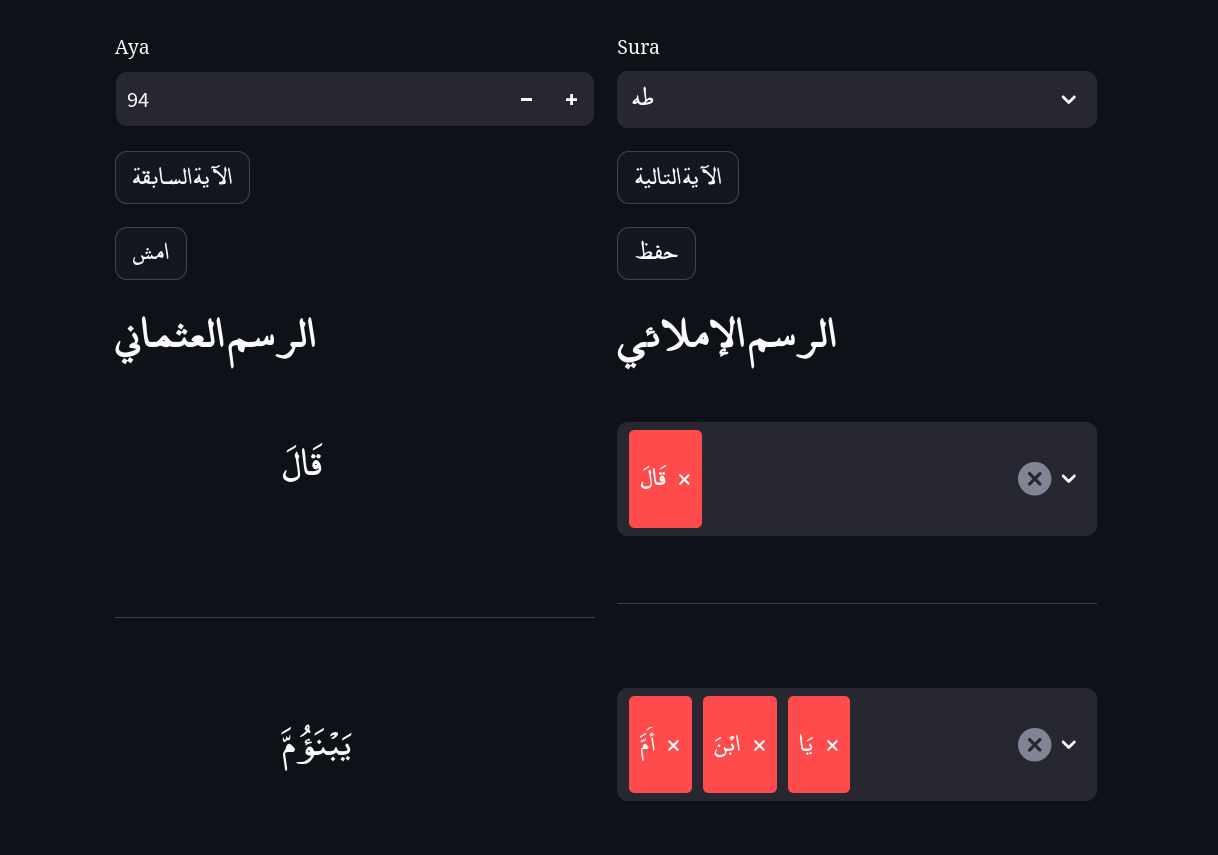
\includegraphics[width=0.8\textwidth]{../figures/imlaey-to-uthmani.png}
\caption{A screenshot of the UI where the user aligns words for both scripts.}
\label{fig:alignment-ui}
\end{figure}

\subsection{Observations}

After completing the annotation, we attempted to identify patterns of mismatches between the Imlaey and Uthmani scripts. We found the following patterns, as shown below:

\begin{table}[H]
\centering
\begin{tabular}{|l|l|l|}
\hline
\textbf{Imlaey Script} & \textbf{Uthmani Script} & \textbf{(Surah, Ayah)} \\
\hline
\arb{يَا ابْنَ أُمَّ} & \arb{يَبْنَؤُمَّ} & (20, 94) \\
\hline
\arb{وَأَن لَّوِ} & \arb{وَأَلَّوِ} & (72, 16) \\
\hline
\end{tabular}
\caption{Examples of script mismatches}
\label{tab:mismatches}
\end{table}

Specifically, we found that Imlaey words starting with certain patterns, along with the following word, map to a single Uthmani word.

\begin{table}[H]
\centering
\begin{tabular}{|l|l|}
\hline
\textbf{Imlaey Word Start} & \textbf{Count in the Holy Quran} \\
\hline
\arb{يَا} & 350 \\
\hline
\arb{وَيَا} & 11 \\
\hline
\arb{هَا} & 4 \\
\hline
\end{tabular}
\caption{Common Imlaey word patterns}
\label{tab:patterns}
\end{table}

\subsection{Imlaey to Uthmani Algorithm}

Based on these observations, we created an algorithm that performs a lookup for these patterns to align both scripts. This resulted in the \texttt{quran-transcript}\footnote{\url{https://github.com/obadx/quran-transcript}} Python package. With a simple \texttt{pip} installation command, the conversion is functional:


\begin{listing}[H]
\begin{minted}[escapeinside=``]{python}
from quran_transcript import search, Aya

imlaey_text = `\pythonarb{فأخرج به من الثمرات رزقا لكم}`
results = search(
    imlaey_text,
    start_aya=Aya(2, 13),
    window=20,
    remove_tashkeel=True
)

uthmani_script = results[0].uthmani_script
print(uthmani_script)
# Output: `\pythonarb{فَأَخْرَجَ بِهِۦ مِنَ ٱلثَّمَرَٰتِ رِزْقًۭا لَّكُمْ}`
\end{minted}
\caption{Usage example with escaped Arabic}
\label{code:example-escaped}
\end{listing}




% ------------------------------------------------------------------------------------------------------------


\section{Quran Phonetic Script Construction}

The Quran Phonetic Script is a set of letters and attributes (\arb{صفات}) that describes what the Holy Quran's reciters \textbf{actually} said. It was designed to capture all recitation rules, including all Tajweed rules (except Ishmam \arb{إشمام} and pausing with rawm \arb{روم} or \arb{إشمام}) and Sifat. This script is composed of 11 levels:

\begin{itemize}
\item \texttt{phonemes} level: Designed to capture pronunciation of letters like baa (\arb{ب}) and diaractization like (fatha, damma and kasra).
\item \texttt{sifat} level: Consisting of 10 levels to capture the attribute of articulation (\arb{صفة}) for every phoneme group.
\end{itemize}

We built this script based on \texttt{Hafs} (\arb{رواية حفص}) and incorporated all the different ways of reciting for \texttt{Hafs}. For example, the length of Madd Almunfasil can be (2, 3, 4, or 5 beats). Other variations can be found here \ref{sec:hafs_ways}.

\subsection{Phonemes Level}

The phoneme level has specific features, which are summarized as:

\begin{enumerate}
\item \textbf{Madd Representation}:
\begin{itemize}
\item Normal Madd appears as consecutive madd symbols (e.g., 4-beat Madd: \arb{اااا}).
\item Madd al-Leen is represented with multiple waw/yaa symbols.
\end{itemize}

\item \textbf{Ghunnah}:
\begin{itemize}
\item Stressed Ghunnah for noon (e.g., \arb{النون المشددة}) is represented as three consecutive noon symbols (\arb{ننن}).
\item Ikhfa is represented as three consecutive noon\_mokhfah (\arb{ںںں}) or meem\_mokhfah (\arb{۾۾۾}).
\end{itemize}

\item \textbf{Idgham Handling}:
\begin{itemize}
\item Idgham for sakin noon with yaa is represented by consonant doubling (e.g., \arb{مَن يَعْمَلْ} → \arb{مَنيييَعمَل}).
\end{itemize}

\item \textbf{Special Cases}:
\begin{itemize}
\item Sakin: No following vowel symbol.
\item Imala: Represented by fatha\_momala and alif\_momala.
\item Rawm: Represented by the dama\_mokhtalasa marker.
\end{itemize}
\end{enumerate}


\begin{table*}[h]
\centering
\caption{Examples of Uthmani to Phonetic Script Conversion with Sifat Attributes}
\label{tab:examples_with_sifat}
\scriptsize
\setlength{\tabcolsep}{3pt}
\begin{tabular}{@{}>{\centering\arraybackslash}m{1.2cm} >{\centering\arraybackslash}m{1.5cm} *{10}{>{\centering\arraybackslash}m{0.7cm}@{}}}
\toprule
\textbf{Uthmani} & \textbf{Phonetic} & 
\textbf{H/J} & 
\textbf{S/R} & 
\textbf{T/T} & 
\textbf{Itb} & 
\textbf{Saf} & 
\textbf{Qal} & 
\textbf{Tik} & 
\textbf{Taf} & 
\textbf{Ist} & 
\textbf{Gho} \\
\cmidrule(lr){1-1} \cmidrule(lr){2-2} \cmidrule(lr){3-12}
\arb{أَ} & \arb{ءَ} & jahr & shd & mrq & mnf & no & nql & nkr & ntf & nst & nmg \\
\arb{تُ} & \arb{تُ} & hams & shd & mrq & mnf & no & nql & nkr & ntf & nst & nmg \\
\arb{حَـ} & \arb{حَ} & hams & rkh & mrq & mnf & no & nql & nkr & ntf & nst & nmg \\
\arb{ـٰٓ} & \arb{اااااا} & hams & rkh & mrq & mnf & no & nql & nkr & ntf & nst & nmg \\
\arb{جُّ} & \arb{ججُ} & jahr & shd & mrq & mnf & no & nql & nkr & ntf & nst & nmg \\
\arb{وٓ} & \arb{ۥۥۥۥۥۥ} & jahr & rkh & mrq & mnf & no & nql & nkr & ntf & nst & nmg \\
\arb{نِّ} & \arb{ننننِ} & jahr & btw & mrq & mnf & no & nql & nkr & ntf & nst & mg \\
\arb{ى} & \arb{ۦۦ} & jahr & rkh & mrq & mnf & no & nql & nkr & ntf & nst & nmg \\
\bottomrule
\end{tabular}

\vspace{2mm}
\begin{center}  % Centering wrapper added here
\scriptsize
Phonetization of word (\arb{أَتُحَٰٓجُّوٓنِّى}) \\
\textbf{Attribute Abbreviations:} \\
H/J: Hams/Jahr \quad S/R: Shidda/Rakhawa \quad T/T: Tafkheem/Taqeeq \quad Itb: Itbaq \\
Saf: Safeer \quad Qal: Qalqla \quad Tik: Tikraar \quad Taf: Tafashie \quad Ist: Istitala \quad Gho: Ghonna \\

\textbf{Value Abbreviations:} \\
shd: shadeed \quad rkh: rikhw \quad btw: between \quad mrq: moraqaq \\
mof: mofakham \quad mnf: monfateh \quad mtb: motbaq \quad no: no\_safeer \\
nql: not\_moqalqal \quad nkr: not\_mokarar \quad ntf: not\_motafashie \\
nst: not\_mostateel \quad nmg: not\_maghnoon \quad mg: maghnoon
\end{center}  % End of centering wrapper
\end{table*}



We only care about pronounced phonemes of letters. If a letter is dropped or not pronounced, we will omit it. For example, we drop the Wasl Hamza (\arb{همزة الوصل}) when it appears in a context like: (\arb{بِسْمِ اللَّهِ}).

\subsubsection{Disconnected Letters}

Disconnected letters (\arb{الحروف المقطعة}) are letters that are pronounced as individual alphabets one by one. For example: (\arb{الٓمٓ}) is pronounced (\arb{أَلِفْ لَآم مِّيٓمْ}). There are 14 forms of these disconnected letters, so we must separate them according to their actual pronunciation.

\subsubsection{Madd (\arb{المد})}

There are three types of elongation (\arb{مد}):
\begin{itemize}
    \item \textbf{Madd Alif} (\arb{مد ألف}): Fatha followed by alif (\arb{ا})
    \item \textbf{Madd Waw} (\arb{مد بالواو}): Damma followed by waw (\arb{و})
    \item \textbf{Madd Yaa} (\arb{مد ياء}): Kasra followed by Yaa (\arb{ي})
\end{itemize}

These Madd types have different lengths relative to the natural Madd (\arb{المد الطبيعي}). We created special symbols to denote each Madd type:

\begin{itemize}
    \item \textbf{Madd Alif} is denoted by multiple alif symbols (\arb{ا})
    \item \textbf{Madd Waw} is denoted by multiple small\_waw symbols, designated as \texttt{waw\_madd} (\arb{ۥ})
    \item \textbf{Madd Yaa} is denoted by multiple small\_yaa symbols, designated as \texttt{yaa\_madd} (\arb{ۦ})
\end{itemize}



\paragraph{Normal Madd (\arb{المد الطبيعي})}

Normal Madd is the type of elongation pronounced at its standard length without excessive prolongation. We denote it by doubling the respective \texttt{madd} phonemes. The example below \ref{tab:ex_normal_madd} shows all three types of Madd in a single word.

\begin{longtable}{|c|c|}
\caption{The table demonstrates the three types of normal Madd: Madd Alif (\arb{اا}), Madd Yaa (\arb{ۦۦ}), and Madd Waw (\arb{ۥۥ}), each represented with two symbols to indicate a two-beat elongation.}
\label{tab:ex_normal_madd}\\
\hline
\textbf{Uthmani Script} & \textbf{Phonetic Script} \\ \hline
\endfirsthead
\hline
\arb{نُوحِيهَا} & \arb{نُۥۥحِۦۦهَاا} \\ \hline
\end{longtable}

\paragraph{Madd Small Silah (\arb{مد الصلة الصغرى})}

Along with Normal Madd, Small Silah Madd (\arb{مد الصلة الصغرى}) follows the same representation rules. For example \ref{tab:ex_small_silah}:

\begin{longtable}{|c|c|}
\caption{The table shows Small Silah Madd along with noon mushaddad denoted as 3 repeated \texttt{noon} (\arb{ن}) with a special qalqala sign: (\arb{ڇ}) for letter jeem (\arb{ج}).}
\label{tab:ex_small_silah}\\
\hline
\textbf{Uthmani Script} & \textbf{Phonetic Script} \\ \hline
\endfirsthead
\hline
\arb{إِنَّهُۥ عَلَىٰ رَجْعِهِۦ لَقَادِرٌ} & \arb{ءِننننَهُۥۥ عَلَاا رَجڇعِهِۦۦ لَقَاادِر} \\ \hline
\end{longtable}

\paragraph{Madd Al-'Iwad (\arb{مد العوض})}

In addition, Madd Al-'Iwad (\arb{مد العوض}) is represented as shown in \ref{tab:ex_alewad}:

\begin{longtable}{|c|c|}
\caption{The table shows Madd Al-'Iwad (\arb{مد العوض}) using the same notation as normal Madd (\arb{المد الطبيعي}) for Madd alif. This type of Madd occurs when a tanween fatha on a final letter is replaced by an alif madd during pause.}
\label{tab:ex_alewad}\\
\hline
\textbf{Uthmani Script} & \textbf{Phonetic Script} \\ \hline
\endfirsthead
\hline
\arb{قَرِيبًا} & \arb{قَرِۦۦبَاا} \\ \hline
\end{longtable}



\subsubsection{Madd Al-Munfasil (\arb{مد المنفصل})}

For Hafs recitation, Madd Al-Munfasil can be elongated for 2, 3, 4, or 5 harakat, where a haraka here is represented as half of a normal Madd when followed by a hamza (\arb{ء}) not in the same word, as shown in the example \ref{tab:ex_monfasel}:

\begin{longtable}{|c|c|}
\caption{The example shows elongation for Madd Al-Munfasil with 4 alif madd phonemes, along with a repeated yaa representing yaa mushaddada (\arb{ياء مشددة}) with both a sakin yaa and a yaa with haraka (damma).}
\label{tab:ex_monfasel}\\
\hline
\textbf{Uthmani Script} & \textbf{Phonetic Script} \\ \hline
\endfirsthead
\hline
\arb{يَٰٓأَيُّهَا} & \arb{يَااااءَييُهَاا} \\ \hline
\end{longtable}


\paragraph{Madd As-Silah Al-Kubra (\arb{مد الصلة الكبرى})}

The same rule is applied to Madd As-Silah Al-Kubra (\arb{مد الصلة الكبرى}). As shown in the example below: \ref{tab:ex_big_silah}

\begin{longtable}{|c|c|}
\caption{The example shows elongation for Madd As-Silah Al-Kubra with 4 madd waw phonemes (\arb{ۥۥۥۥ}).}
\label{tab:ex_big_silah}\\
\hline
\textbf{Uthmani Script} & \textbf{Phonetic Script} \\ \hline
\endfirsthead
\hline
\arb{مَالَهُۥٓ أَخْلَدَهُۥ} & \arb{مَاالَهُۥۥۥۥ ءَخلَدَه} \\ \hline
\end{longtable}

\paragraph{Madd Al-Muttasil (\arb{المد المتصل})}

For Hafs recitation, Madd Al-Muttasil (\arb{مد المتصل}) can be elongated for 2, 3, 4, 5, or (6 at pause only) harakat, where a haraka is represented as half of a normal Madd when followed by a hamza (\arb{ء}) in the same word, as shown in \ref{tab:ex_mottasel}:

\begin{longtable}{|c|c|}
\caption{The example shows elongation for Madd Al-Muttasil (\arb{مد المتصل}) with 4 madd alif phonemes, along with Madd Al-'Iwad (\arb{مد العوض}) at the pause point.}
\label{tab:ex_mottasel}\\
\hline
\textbf{Uthmani Script} & \textbf{Phonetic Script} \\ \hline
\endfirsthead
\hline
\arb{ٱلسَّمَآءِ مَآءً} & \arb{ءَسسَمَااااءِ مَااااءَاا} \\ \hline
\end{longtable}


\paragraph{Madd Al-Lazim (\arb{المد اللازم})}

Madd Al-Lazim (\arb{المد اللازم}) is the type of Madd where a Madd letter is followed by a Sakin letter (\arb{حرف ساكن}) in the same word and is elongated for 6 harakat (\arb{6 حركات}), where a haraka is represented as half of a normal Madd.

\begin{longtable}{|c|c|}
\caption{The table shows an example of Madd Al-Lazim (\arb{المد اللازم}) with Madd alif elongated for 6 harakat, along with Madd Al-'Arid Li-S-Sukun (\arb{مد العرض للسكون}) represented with 4 harakat.}
\label{tab:ex_lazem}\\
\hline
\textbf{Uthmani Script} & \textbf{Phonetic Script} \\ \hline
\endfirsthead
\hline
\arb{ٱلضَّآلِّينَ} & \arb{ءَضضَااااااللِۦۦۦۦنَ} \\ \hline
\end{longtable}



\paragraph{Madd Al-\arb{عارض} Li-S-\arb{سكون} (\arb{مد العارض للسكون})}

Madd Al-\arb{عارض} Li-S-\arb{سكون} is the madd that occurs when pausing after a normal madd with a sakin letter. This madd is elongated for 2, 4, or 6 harakat, where the haraka is represented as half of the normal madd length, as shown in \ref{tab:ex_lazem}:

\paragraph{Madd Al-\arb{لين} (\arb{مد اللين})}

Madd Al-\arb{لين} (\arb{مد اللين}) occurs when pausing after a \arb{ياء} (\arb{ي}) or \arb{واو} (\arb{و}) that is preceded by a fatha and followed by a sakin letter. This madd is elongated for 2, 4, or 6 harakat, where a haraka is represented as half of the normal madd length \ref{tab:ex_leen}. We do not create special phonemes for this rule as we did with other madd types because \arb{لين} represents an elongation of existing \arb{واو} (\arb{و}) or \arb{ياء} (\arb{ي}) phonemes rather than introducing new phonemes.

For a 4-haraka madd, we denote this with (number\_of\_harakat - 1) symbols. This approach accounts for cases of Madd Al-\arb{لين} in the middle of recitation (like \arb{وَٱلْمَيْسِرِ}) as well as at pause positions, maintaining consistency in the phonetic script. Table \ref{tab:ex_leen} shows an example of Madd Al-\arb{لين}:

\begin{longtable}{|c|c|}
\caption{The example shows two forms of madd: the first is normal madd followed by Madd Al-\arb{لين} with 4 harakat (each haraka being half of normal madd), denoted with 3 \arb{ياء} (\arb{ي}) symbols.}
\label{tab:ex_leen}\\
\hline
\textbf{Uthmani Script} & \textbf{Phonetic Script} \\ 
\hline
\endfirsthead
\hline
\arb{لِإِيلَٰفِ قُرَيْشٍ} & \arb{لِءِۦۦلَاافِ قُرَيييش} \\
\hline
\end{longtable}


\subsubsection{Ghunnah (\arb{العنة})}

We consider tanween here as a haraka (fatha, damma, or kasra) followed by a sakin noon (\arb{نون ساكنة}), so we do not need to define separate rules for noon (\arb{ن}) and tanween.

\paragraph{Noon Mushaddadah (\arb{النون المشددة})}

We first attempted to measure the relative timing of a sakin noon alone (\arb{النون الساكنة المظهرة}) and compare it to an elongated noon (noon with shaddah - \arb{نون مشددة}). We found that the elongated noon is approximately 3 to 4 times longer than the sakin noon, so we defined the elongated noon as equivalent to 3 sakin noon repetitions. Example in table: \ref{tab:ex_noon_moshadada}

\begin{longtable}{|c|c|}
\caption{The table shows how Ghunnah disassembly of noon with shaddah (\arb{نون مشددة}) is represented as 3 repetitive noon (\arb{ن}) symbols.}
\label{tab:ex_noon_moshadada}\\
\hline
\textbf{Uthmani Script} & \textbf{Phonetic Script} \\ 
\hline
\endfirsthead
\hline
\arb{إِنَّ} & \arb{ءِننن} \\
\hline
\arb{شَىْءٍ نُّكُرٍ} & \arb{شَيءِننننُكُر} \\
\hline
\end{longtable}

\paragraph{Meem Mushaddadah (\arb{الميم المشددة})}

As we have done with Noon Mushaddadah, we applied the same principle to Meem Mushaddadah (elongated meem). We found the same result: Meem Mushaddadah is approximately 3 to 4 times longer than a regular sakin meem (\arb{ميم ساكنة مظهرة}). We denote Meem Mushaddadah as 3 repeated meem symbols, as shown in the examples: \ref{tab:ex_meem_moshadda}

\begin{longtable}{|c|c|}
\caption{The table shows how Ghunnah disassembly of meem with shaddah (\arb{ميم مشددة}) is represented as 3 repeated meem (\arb{م}) symbols.}
\label{tab:ex_meem_moshadda}\\
\hline
\textbf{Uthmani Script} & \textbf{Phonetic Script} \\ 
\hline
\endfirsthead
\hline
\arb{أَمَّا} & \arb{ءَممممَاا} \\
\hline
\arb{خَيْرٍ مِّن} & \arb{خَيرِممممِن} \\
\hline
\end{longtable}

\paragraph{Ikhfaa for Noon (\arb{إخفاء النون الساكنة})}

Ikhfaa for sakin noon (\arb{إخفاء النون الساكنة}) occurs when a sakin noon (\arb{نون ساكنة}) or tanween is followed by any of the Ikhfaa letters: (\arb{ص، ذ، ث، ك، ج، ش، ق، س، د، ط، ز، ت، ض، ظ، ف}). We denote this by replacing the noon with three `noon_mokhfaa` symbols (\arb{ں}), as shown in the example \ref{tab:ex_noon_mokhfaa}:

\begin{longtable}{|c|c|}
\caption{The table shows the representation of noon mokhfaa (\arb{نون مخفاة}) as three dotless noon symbols (\arb{ں}).}
\label{tab:ex_noon_mokhfaa}\\
\hline
\textbf{Uthmani Script} & \textbf{Phonetic Script} \\ 
\hline
\endfirsthead
\hline
\arb{مِن صَلْصَٰلٍ} & \arb{مِںںںصَلصَاااال} \\
\hline
\end{longtable}



\paragraph{Idgham for Noon with Yaa and Waw (\arb{إدغام النون الساكنة مع الياء والواو})}

The Idgham rule is defined as pronouncing two consecutive letters as the second letter with shadda (stress) according to Ibn Al-Jazari \cite{ibnaljazri_alnashr}. Therefore, we simply delete the noon (\arb{ن}) and replace it with a yaa (\arb{ي}) or waw (\arb{و}).

As with Noon Mushaddadah and Meem Mushaddadah, we represent the resulting stressed yaa or waw with two repetitions rather than three. This maintains consistency with our representation of Madd Al-\arb{لين} and follows the convention that a stressed letter (\arb{مشدد}) is represented by both a sakin and mutaharrik (\arb{متحرك}) form. Table \ref{tab:ex_idghaam_yaa_with_noon} shows examples of different forms of yaa:

\begin{longtable}{|c|c|}
\caption{This table demonstrates different representations of yaa. The first row shows Idgham of yaa with sakin noon (\arb{النون الساكنة}) represented by replacing the noon with two yaa symbols. The second row shows yaa with shadda at pause represented with two yaa symbols. The third row shows Madd Al-\arb{لين} with 4 harakat represented by 3 yaa symbols.}
\label{tab:ex_idghaam_yaa_with_noon}\\
\hline
\textbf{Uthmani Script} & \textbf{Phonetic Script} \\ 
\hline
\endfirsthead
\hline
\arb{مَن يَعْمَلْ} & \arb{مَيييَعمَل} \\
\hline
\arb{ٱلْحَىِّ} & \arb{ءَلحَيي} \\
\hline
\arb{قُرَيْشٍ} & \arb{قُرَيييش} \\
\hline
\end{longtable}

\paragraph{Ikhfaa for Meem (\arb{إخفاء الميم الساكنة})}

Ikhfaa for sakin meem (\arb{إخفاء الميم الساكنة}) occurs when a sakin meem (\arb{ميم ساكنة}) is followed by a baa (\arb{ب}). Additionally, when a sakin noon or tanween is followed by baa, it is defined in Tajweed literature as Iqlab (\arb{إقلاب}). We represent both cases with three `meem_mokhfah` symbols (\arb{۾}). Table \ref{tab:ex_ikhfaa_meem} shows how this rule is applied:

\begin{longtable}{|c|c|}
\caption{The first row represents the Iqlab rule (\arb{الإقلاب}), which is denoted by replacing the noon with 3 `meem_mokhfah` symbols (\arb{۾}) and \arb{(ڇ)} donates Qalqala. The second row shows the rule of Ikhfaa for sakin meem with baa (\arb{إخفاء الميم الساكنة}), represented by 3 `meem_mokhfah` symbols (\arb{۾}).}
\label{tab:ex_ikhfaa_meem}\\
\hline
\textbf{Uthmani Script} & \textbf{Phonetic Script} \\ 
\hline
\endfirsthead
\hline
\arb{مِنۢ بَعْدِ} & \arb{مِ۾۾۾بَعدڇ} \\
\hline
\arb{تَرْمِيهِم بِحِجَارَةٍ} & \arb{تَرمِۦۦهِ۾۾۾بِحِجَاارَه} \\
\hline
\end{longtable}


\subsubsection{Idgham (\arb{الإدغام})}

There are two types of merging (Idgham) in Arabic:

\begin{itemize}
\item \textbf{Full Merging (\arb{إدغام كامل})}: When two letters follow each other and are pronounced as only the second letter, but stressed. Example: (\arb{قَد تَّبَيَّنَ}) is pronounced as (\arb{قَتتَبَييَن}) where the letter daal is completely not pronounced.
\item \textbf{Partial Merging (\arb{إدغام ناقص})}: When two letters follow each other and the articulation point (makhraj) of the first letter is lost but its attributes (sifat) remain. Example: (\arb{بَسَطْتَ}) is pronounced the same (\arb{بَسَطَت}).
\end{itemize}

\subsubsection{Sakin Letter (\arb{الحرف الساكن})}

A sakin letter is represented in the Uthmani script in three forms:

\begin{enumerate}
\item A letter followed by sukun (\arb{سُكُون}): '\arb{ْ}'
\item A letter with shaddah (\arb{شَدَّة}), which represents a stressed letter composed of two identical letters: the first is sakin and the second has a haraka (fatḥah, ḍammah, or kasrah). Example: (\arb{بَّ}) → (\arb{ببَ})
\item A letter that is not followed by any haraka (short vowel) or any special symbol, which occurs in Idgham and with madd letters.
\end{enumerate}

We denote a sakin letter by the absence of any following vowel diacritic.

\subsubsection{Pausing (\arb{وَقْف})}

At a pause (\arb{وَقْف}), we make the final letter sakin (\arb{سَاكِن}) by removing any vowel diacritic. See examples in: \ref{tab:ex_idghaam_yaa_with_noon} and other relevant tables.




\subsubsection{Hamzat Al-Wasl (\arb{همزة الوصل})}

Hamzat Al-Wasl (\arb{همزة الوصل}) (\arb{ٱ}) is defined in Tajweed as a hamza added to avoid beginning with a sakin letter \cite{sweed2021}. It is elided during continuous recitation and is only pronounced at the beginning.

The vowel following Hamzat Al-Wasl (fatha, damma, or kasra) depends on the word type:

\begin{itemize}
\item For nouns beginning with Alif-Lam at-ta'reef (\arb{ال التعريف}), the hamza is followed by fatha.
\item For proper nouns, the hamza is followed by kasra.
\item For verbs: the vowel depends on the third root letter:
\begin{itemize}
    \item Damma: hamza is followed by non-transient damma
    \item Fatha, kasra, or transient damma: hamza is followed by kasra
\end{itemize}
\end{itemize}

\textbf{Transient damma} refers to a damma that is not original but results from a temporary grammatical state. For example, the word (\arb{ٱمْشُوا۟}) has a damma on its third letter, but the verb originates from (\arb{ٱمْشِ}) where the third letter (\arb{ش}) has kasra.

\begin{longtable}{|c|c|c|c|}
\caption{This table shows different forms of Hamzat Al-Wasl (\arb{ٱ}). The first and second rows demonstrate beginning with hamza followed by fatha due to (\arb{ال}) at-ta'reef. The third row shows beginning with hamza followed by kasra for a proper noun. The 4th, 5th, and 6th rows show verbs beginning with hamza followed by kasra because the third radical has fatha, kasra, or transient damma. The last row shows beginning with hamza followed by damma because the third radical has a non-transient damma.}
\label{tab:ex_hamzat_wasl}\\
\hline
\textbf{Uthmani Script} & \textbf{Phonetic Script} & \textbf{Word Type} & \textbf{Hamzat Wasl Vowel} \\ 
\hline
\endfirsthead
\hline
\arb{ٱلْكِتَٰبُ} & \arb{ءَلكِتَاااابڇ} & Noun beginning with (\arb{ال}) & fatha \\
\hline
\arb{ٱللَّهِ} & \arb{ءَللَااااه} & Proper Noun beginning with (\arb{ال}) & fatha \\
\hline
\arb{ٱسْتِكْبَارًۭا} & \arb{ءِستِكبَاارَاا} & Proper Noun & kasra \\
\hline
\arb{ٱرْكَب} & \arb{ءِركَبڇ} & Verb (3rd letter has fatha) & kasra \\
\hline
\arb{ٱصْبِرْ} & \arb{ءِصبِر} & Verb (3rd letter has kasra) & kasra \\
\hline
\arb{ٱمْشُوا۟} & \arb{ءِمشُۥۥ} & Verb (3rd letter has transient damma) & kasra \\
\hline
\arb{ٱرْكُضْ} & \arb{ءُركُض} & Verb (3rd letter has non-transient damma) & damma \\
\hline
\end{longtable}

\textbf{Important Note}: We rely on Dukes's work \cite{dukes2010morphological} for determining word types (nouns, verbs, and particles). Without this foundational research, annotating the Holy Quran's words would require at least a year of dedicated effort, highlighting the critical importance of open-source linguistic resources.

\paragraph{Meeting Two Hamzas (Second One is Sakin) (\arb{التقاء همزتان والثانية منهما ساكنة})}

After converting Hamzat Wasl to a pronounced hamza, certain cases occur where two hamzas meet and the second one is sakin (consonant). In such cases, the second hamza is converted to a madd letter matching the vowel (haraka) of the first hamza \cite{sweed2021}. Table \ref{tab:ex_meeting_two_hamza} illustrates this process:

\begin{longtable}{|c|c|c|}
\caption{The table shows the conversion process for verbs that begin with two connected hamzas. The first stage converts Hamzat Wasl to a hamza followed by kasra or damma. The second stage converts the second hamza to either waw\_madd (\arb{ۥ}) or yaa\_madd (\arb{ۦ}), depending on the vowel of the first hamza. We maintain our established representation where normal madd is represented by two symbols: (\arb{اا}) for madd\_alif, (\arb{ۦۦ}) for madd\_yaa, and (\arb{ۥۥ}) for madd\_waw.}
\label{tab:ex_meeting_two_hamza}\\
\hline
\textbf{Uthmani Script} & \textbf{Converting Hamzat Wasl} & \textbf{Final Conversion} \\ 
\hline
\endfirsthead
\hline
\arb{ٱؤْتُمِنَ} & \arb{ءُءْتُمِن} & \arb{ءُۥۥتُمِن} \\
\hline
\arb{ٱئْتُونِى} & \arb{ءِءْتُۥۥنِۦۦ} & \arb{ءِۦۦتُۥۥنِۦۦ} \\
\hline
\end{longtable}




\subsubsection{Meeting Two Sakin Letters (\arb{التقاء الساكنين})}

In Arabic language and the Holy Quran, two sakin letters (\arb{الحرفان الساكنان}) cannot meet consecutively except at pause (\arb{وقف}), such as pausing on the word (\arb{ٱلْأَرْضِ}) where the final two letters are sakin. To resolve this meeting, three approaches may be employed:

\begin{itemize}
\item Eliminate the first letter
\item Elongate the first letter
\item Diacritize the second letter with a vowel (fatha, damma, or kasra)
\end{itemize}

Muslim scholars have simplified this task by comprehensively annotating these rules within the Uthmani script, except for two specific cases:
\begin{itemize}
\item When the first letter is (alif, waw, or yaa): we eliminate the first letter
\item When the first letter is tanween: we convert the tanween to a noon (\arb{ن}) followed by kasra
\end{itemize}

Table \ref{tab:ex_two_saken} shows how we apply this rule in our phonetization process:

\begin{longtable}{|c|c|}
\caption{The table demonstrates how we resolve the meeting of two sakin letters. The first row shows the meeting of alif (\arb{ا}) from the word (\arb{قَالَا}) with the lam (\arb{ل}) of the word (\arb{ٱلْحَمْدُ}). In the resulting phonetic script, the alif was deleted. Note that normal madd in (\arb{قَالَ}) is represented by two alif (\arb{اا}), and qalqala in the letter daal (\arb{د}) is represented by (\arb{ڇ}). The second example shows the meeting of tanween from (\arb{نُوحٌ}) with the sakin baa (\arb{ب}) of the word (\arb{ٱبْنَهُۥ}), resulting in the conversion of tanween to noon with kasra. Note also that normal madd waw is represented with two (\arb{ۥۥ}) and qalqala for baa (\arb{ب}) with (\arb{ڇ}).}
\label{tab:ex_two_saken}\\
\hline
\textbf{Uthmani Script} & \textbf{Phonetic Script} \\ 
\hline
\endfirsthead
\hline
\arb{وَقَالَا ٱلْحَمْدُ} & \arb{وَقَاالَ لحَمدڇ} \\
\hline
\arb{نُوحٌ ٱبْنَهُۥ} & \arb{نُۥۥحُنِ بڇنَه} \\
\hline
\end{longtable}

\subsubsection{Shadda (\arb{التشديد})}

Shadda (\arb{ّ}) indicates that a letter is doubled or geminated. We represent this by repeating the letter twice, as shown in \ref{tab:ex_tasheel}.

\subsubsection{Pausing (\arb{الوقف})}

Several rules apply at pause (\arb{وقف}):

\begin{itemize}
\item Vowels (harakat) such as fatha, damma, and kasra are elided, meaning the final letter becomes sakin (\arb{ساكن}).
\item Small Silah Madd is elided.
\item Taa marboota (\arb{ة}) is converted to haa (\arb{ه}).
\end{itemize}

\subsubsection{Qalqala (\arb{القلقة})}

Qalqala (\arb{قلقة}) is defined in tajweed as: "a small sound is followed by on one the letter (\arb{ق - ط - ب - ج - د}) if one of them is sakin (\arb{ساكن}) either in between words (\arb{وصلا}) or at pause (\arb{وقفا})" \cite{AlHamad2008}. We denote this small sound as (\arb{ڇ}) like in table \ref{tab:ex_two_saken}.

\subsubsection{Imala (\arb{الإمالة})}

Imala (\arb{إمالة}) is defined in Tajweed as "pronouncing a fatha somewhere between a fatha and a kasra, and an alif somewhere between an alif and a yaa" \cite{sweed2021}. We denote a fatha with imala as `fatha_momala` (\arb{۪}) and an alif with imala with two `alif_momala` symbols (\arb{ــ}), similar to the representation of Normal Madd. Table \ref{tab:ex_imala} provides an example:

\begin{longtable}{|c|c|}
\caption{The table shows how we represent fatha with imala as (\arb{۪}) and alif with imala as (\arb{ــ}). The letter jeem (\arb{ج}) also exhibits qalqala, denoted by (\arb{ڇ}).}
\label{tab:ex_imala}\\
\hline
\textbf{Uthmani Script} & \textbf{Phonetic Script} \\ 
\hline
\endfirsthead
\hline
\arb{مَجْر۪ىٰهَا} & \arb{مَجڇر۪ــهَاا} \\
\hline
\end{longtable}

\subsubsection{Tasheel (\arb{التسهيل})}

Tasheel is defined in Tajweed as "pronouncing a hamza (\arb{ء}) with a quality intermediate between a full hamza and the following madd letter, similar to an intermediate vowel (\arb{حركة}) between fatha, damma, and kasra" \cite{sweed2021}. We denote this facilitated hamza with the symbol `hamza_mosahala` (\arb{ٲ}). Table \ref{tab:ex_tasheel} provides an example:

\begin{longtable}{|c|c|}
\caption{The table shows a hamza with Tasheel denoted by (\arb{ٲ}), along with the disassembly of the letter yaa (\arb{ي}) with shaddah (\arb{ّ}) into two yaa symbols.}
\label{tab:ex_tasheel}\\
\hline
\textbf{Uthmani Script} & \textbf{Phonetic Script} \\ 
\hline
\endfirsthead
\hline
\arb{ءَا۬عْجَمِىٌّ} & \arb{ءَٲعجَمِيي} \\
\hline
\end{longtable}

\subsubsection{Sakt (\arb{السكت})}

Sakt is defined in tajweed by "cutting voice without releasing of breathe for short period learned from expert reciters" \cite{AlHamad2008}. Sakat happens in a specified positions see: \ref{sec:hafs_ways}. we denote sakt by `sakt` (\arb{ۜ}).



\subsubsection{Implementation}

We implemented our phonetic representation by applying 26 operations. Each operation consists of one or more regular expressions:


\begin{enumerate}
    \item \textbf{DisassembleHrofMoqatta} (\arb{تفكيك حروف مقطعة}): Separates Quranic initials (e.g., \arb{الم، الر}) into individual letters.
    
    \item \textbf{SpecialCases} (\arb{حالات خاصة}): Handles special words like \arb{يبسط} that have different pronunciation forms defined in \texttt{MoshafAttributes}.
    
    \item \textbf{BeginWithHamzatWasl} (\arb{البدء بهمزة الوصل}): Processes words starting with connecting hamza (\arb{ٱ}) and converts it to hamza (\arb{ء}) with appropriate harakah for nouns and verbs.
    
    \item \textbf{BeginWithSaken} (\arb{البدء بساكن}): Manages words beginning with a consonant (sakin) like \arb{لْيَقْطَعْ}, as Arabic doesn't start utterances with consonants.
    
    \item \textbf{ConvertAlifMaksora} (\arb{تحويل الألف المقصورة}): Converts \arb{ى} in Uthmani script to either yaa (\arb{ي}) or alif (\arb{ا}) based on context.
    
    \item \textbf{NormalizeHmazat} (\arb{توحيد الهمزات}): Standardizes hamza forms (\arb{أ إ ؤ ئ}) to \arb{ء}.
    
    \item \textbf{IthbatYaaYohie} (\arb{إثبات ياء يحيى}): Handles words like \arb{يُحْىِۦ} where two yaa letters occur - resolves conflicts when pausing on words with consecutive consonants (\arb{التقاء الساكنين}) by adding another yaa at end.
    
    \item \textbf{RemoveKasheeda} (\arb{إزالة الكشيدة}): Deletes elongation marks (\arb{ـــ}) from text.
    
    \item \textbf{RemoveHmzatWaslMiddle} (\arb{إزالة همزة الوصل الوسطية}): Removes connecting hamza (\arb{ٱ}) in non-initial positions.
    
    \item \textbf{RemoveSkoonMostadeer} (\arb{حذف الحرف الذي فوقع سكون مستدير}): Eliminates letters with circular sukoon diacritics like alif in \arb{جَمَعُوا۟}.
    
    \item \textbf{SkoonMostateel} (\arb{سكون مستطيل}): Removes alif with elongated sukoon mid-word and adds it at the end during pauses (\arb{وقف}).
    
    \item \textbf{MaddAlewad} (\arb{مد العوض}): Removes alif after tanween fatha mid-word and adds alif while removing tanween at pause positions (\arb{وقف}).
    
    \item \textbf{WawAlsalah} (\arb{واو الصلاة}): Replaces letter waw (\arb{و}) with small alif above combined with alif.
    
    \item \textbf{EnlargeSmallLetters} (\arb{تكبير الحروف الصغيرة}): Resizes miniature Arabic letters to standard proportions.
    
    \item \textbf{CleanEnd} (\arb{تنظيف النهاية}): Removes redundant diacritics and spaces at word endings.
    
    \item \textbf{NormalizeTaa} (\arb{توحيد التاء}): Converts \arb{ة} (taa marbuta) to \arb{ت} or \arb{ه} based on context, and converts final \arb{ة} to haa (\arb{ه}).
    
    \item \textbf{AddAlifIsmAllah} (\arb{إضافة ألف اسم الله}): Inserts compensatory alif in derivatives of "\arb{الله}".
    
    \item \textbf{PrepareGhonnaIdghamIqlab} (\arb{تهيئة الغنة والإدغام والإقلاب}): Preprocesses text for nasalization, assimilation, and conversion rules.
    
    \item \textbf{IltiqaaAlsaknan} (\arb{التقاء الساكنين}): Resolves consecutive consonants by inserting vowels.
    
    \item \textbf{DeleteShaddaAtBeginning} (\arb{حذف الشدة في البداية}): Removes shadda (\arb{ّ}) from word-initial letters.
    
    \item \textbf{Ghonna} (\arb{غنة}): Applies nasalization during pronunciation of sakin noon and tanween.
    
    \item \textbf{Tasheel} (\arb{تسهيل}): Adds a letter representing alif with tasheel easing.
    
    \item \textbf{Imala} (\arb{إمالة}): Converts fatha with imala to \texttt{fatha\_momala} phoneme and alif with imala to \texttt{alif\_momala} phoneme.
    
    \item \textbf{Madd} (\arb{مد}): Adds madd symbols for all madd types, inserting \texttt{madd\_alif} (\arb{ا}), \texttt{madd\_waw} (\arb{ۥ}), and \texttt{madd\_yaa} (\arb{ۦ}).
    
    \item \textbf{Qalqla} (\arb{قلقة}): Adds echoing effect to \arb{ق, ط, ب, ج, د} letters with sukoon.
    
    \item \textbf{RemoveRasHaaAndShadda} (\arb{إزالة رأس الحاء علامة السكون}): Deletes sukoon diacritic marks.
\end{enumerate}











\section{Sifat Level}

Sifat (\arb{صفة}), or in English, attributes of articulation, form a foundational component of our phonetic representation. We based our classification on the classical scholarship of Ibn Al-Jazari. While Ibn Al-Jazari enumerated 17 sifat \cite{AlJazariyyahSwaid}, we have excluded 4 of them for the following reasons:

\begin{itemize}
\item \textbf{Ismat (\arb{إصمات})}: This is a phonological, not a purely phonetic, property.
\item \textbf{Ithlaq (\arb{إذلاق})}: Similarly, this is a phonological characteristic rather than a phonetic one.
\item \textbf{Leen (\arb{اللين})}: This attribute is already accounted for within the rules of Madd Al-Leen (\arb{مد اللين}).
\item \textbf{Inhiraf (\arb{الانحراف})}: This property explains why the letters lam (\arb{ل}) and raa (\arb{ر}) are classified between shidda (\arb{شدة}) and rakhawa (\arb{رخاوة}), and is thus subsumed by those attributes.
\end{itemize}

We have included the sifa of Al-Ghunnah (\arb{صفة الغنة}), resulting in a system that represents 14 sifat organized into 10 distinct levels, as detailed in table \ref{table:table_sifa_level_def}.

\begin{itemize}
\item \textbf{Hams/Jahr (\arb{الهمس/الجهر})}
\begin{itemize}
  \item \textit{Hams}: Whispered letters requiring breath flow (\arb{ف ح ث ه ش خ ص س ك ت})
  \item \textit{Jahr}: Voiced letters with full the rest of letters
\end{itemize}

\item \textbf{Shidda/Rakhawa (\arb{الشدة/الرخاوة})}
\begin{itemize}
  \item \textit{Shidda}: Complete interruption of sound (\arb{ء ج د ق ط ب ك ت})
  \item \textit{Between Shiddah and Rqkahwa}: in between of both (\arb{ل ن ع م ر})
  \item \textit{Rakhawa}: Continuous airflow the rest of letter.
\end{itemize}

\item \textbf{Tafkheem/Taqeeq (\arb{التفخيم/الترقيق})}
\begin{itemize}
  \item \textit{Tafkheem}: Heavy/thickened pronunciation (\arb{خ ص ض ط ظ غ ق})
  \item \textit{Taqeeq}: Light/thin pronunciation rest of letter with exepsion descripted below
\end{itemize}

\item \textbf{Itbaq (\arb{الإطباق})}
\begin{itemize}
  \item \textit{Motbaq} Letters pronounced with tongue-to-palate contact (\arb{ص ض ط ظ})
  \item \textit{Monfateh} Rest of the letters
\end{itemize}

\item \textbf{Safeer (\arb{الصفير})}
\begin{itemize}
  \item \textit{Safeer} Whistling sound in \arb{س ص ز}
  \item \textit{No Safeer} the rest of the letters
\end{itemize}

\item \textbf{Qalqala (\arb{القلقلة})}
\begin{itemize}
  \item \textit{Moqlqal} Echo effect on \arb{ق ط ب ج د} when bearing sukoon
  \item \textit{Not Moqlqal} the rest of letters
\end{itemize}

\item \textbf{Tikraar (\arb{التكرار})}
\begin{itemize}
  \item \textit{Mokarrar} the Quranic letter (\arb{ر}) is trilled just (like Spanish perro)
  \item \textit{Not Mokarrar} the rest of letters
\end{itemize}

\item \textbf{Tafashie (\arb{التفشي})}
\begin{itemize}
  \item \textit{Motafashie} Sound dispersion characteristic of \arb{ش}
  \item \textit{Not Motafashie} Rest of letters
\end{itemize}

\item \textbf{Istitala (\arb{الاستطالة})}
\begin{itemize}
  \item \textit{Mostateel} sepecial attribute emphatic and pharyngealized for letter (\arb{ض})
  \item \textit{Not Mostateel} Rest of letters
\end{itemize}

\item \textbf{Ghonna (\arb{الغنة})}
\begin{itemize}
  \item \textit{Maghnoon} Nasalization in \arb{ن} and \arb{م}
  \item \textit{Not Maghnoon} The other letters
\end{itemize}
\end{itemize}

Our methodology for transcribing Sifat involves first chunking phonemes by grouping similar phoneme categories and then extracting the Sifat for each phoneme group, as shown in the example \ref{tab:examples_with_sifat}. Subsequently, we extract the Sifat for every group.

The extraction of Sifat is straightforward, with the exception of Tafkheem and Tarqeeq.

\subsubsection{Tafkheem and Tarqeeq (\arb{التفخيم والترقيق})}

Tafkheem (\arb{التفخيم}) is defined as "thickening that affects a phoneme, causing it to fill the entire mouth" \cite{sweed2021}.

In Tajweed, there are 6 levels of Tafkheem and Tarqeeq, ordered from strongest (most mofakham) to weakest (moraqaq):

\begin{enumerate}
\item Mofakham followed by fatha and then madd alif.
\item Mofakham followed by fatha without madd alif.
\item Mofakham followed by damma.
\item Mofakham in a sakin (\arb{ساكن}) state.
\item Mofakham followed by kasra.
\item Moraqaq.
\end{enumerate}

We have formulated these into three labels:

\begin{enumerate}
\item `mofakham` to cover cases 1 to 4.
\item `moraqaq` to cover case 6.
\item `low_mofakham` to cover case 5 for the letters (\arb{غ, خ, ق}), which are monfateh (\arb{منفتح}) and not motbaq (\arb{مطبق}). These letters are weakened by a kasra, unlike motbaq letters such as (\arb{ص, ض, ط, ظ}).
\end{enumerate}

Some phonemes exhibit cases where they can be either moraqaq or mofakham:

\begin{itemize}
\item `madd_alif` (\arb{ا}): Its Tafkheem or Tarqeeq follows that of the preceding phoneme.
\item `noon_mokhfah` (\arb{ں}): Its Tafkheem or Tarqeeq follows that of the subsequent phoneme.
\item `raa` (\arb{ر}) is moraqaq in the following cases:
\begin{itemize}
    \item When followed by a kasra.
    \item When preceded by a sakin yaa (\arb{ياء}).
    \item When it is sakin (\arb{ساكن}) and preceded by a mostafel (\arb{مستفل}) phoneme with a kasra, and not followed by a mosta'lie (\arb{مستعلي}) phoneme.
    \item When it appears after a hamzat wasl (\arb{ٱ}).
\end{itemize}
\end{itemize}

\textbf{Note}: The Mosta'lie (\arb{حروف الاستعلاء}) letters are (\arb{خ, ص, ض, غ, ط, ق, ظ}), and the Mostafel (\arb{مستفل}) letters comprise all others.
% Chapter 4

\chapter{Preparing Dataset} % Main chapter title

\label{Chapter4} % For referencing the chapter elsewhere, use \ref{Chapter4} 

\lhead{Chapter 4. \emph{Preparing Dataset}} % This is for the header on each page - perhaps a shortened title




\section{Introduction}

The data preparation process began with the definition of clear selection criteria. Our objective was to compile recitations from world-class experts to serve as reference models for evaluating Quranic learners. This study focuses exclusively on the Hafs Way (\arb{رواية حفص}) due to its status as the most prevalent recitation method globally.

Acknowledging that manual annotation is prohibitively time-consuming, we developed a data collection pipeline that is approximately 98\% automated. The procedure consists of the following steps:

\begin{enumerate}
\item Selection of a digitized Quranic script as the foundational text.
\item Definition of precise criteria for the \arb{حفص} methodology.
\item Collection of expert recitations.
\item Segmentation of audio at pause points (\arb{وقف}).
\item Transcription of the segmented audio.
\item Data validation using a Tasmeea (\arb{تسميع}) algorithm.
\item Extraction of a phonetic script using our custom Quran Phonetic Script.
\end{enumerate}

For the purposes of this work, a moshaf (\arb{مصحف}) is defined as a complete recitation of the Quran (chapters 1-114) by a single reciter. The statistics of the collected dataset are summarized in Table \ref{tab:all_data_stat}.

\begin{longtable}{|c|c|c|}
\caption{Summary of the proposed dataset. The final collection comprises approximately 848 hours of audio, totaling over 286,000 individual recitation segments.}
\label{tab:all_data_stat}\\
\hline
\textbf{Moshaf ID} & \textbf{Hours} & \textbf{Recitation Count} \\ 
\hline
\endfirsthead
\hline
0.0 & 28.48 & 9,133 \\
\hline
0.1 & 40.31 & 10,764 \\
\hline
0.2 & 49.47 & 9,971 \\
\hline
0.3 & 37.19 & 12,604 \\
\hline
1.0 & 28.41 & 10,939 \\
\hline
2.0 & 51.05 & 9,942 \\
\hline
2.1 & 30.03 & 10,394 \\
\hline
3.0 & 25.19 & 10,444 \\
\hline
4.0 & 29.12 & 10,994 \\
\hline
5.0 & 28.02 & 11,482 \\
\hline
6.0 & 39.39 & 12,435 \\
\hline
7.0 & 28.26 & 9,907 \\
\hline
8.0 & 30.86 & 10,330 \\
\hline
9.0 & 27.95 & 10,642 \\
\hline
11.0 & 24.01 & 10,363 \\
\hline
12.0 & 33.42 & 9,880 \\
\hline
13.0 & 33.99 & 9,377 \\
\hline
19.0 & 30.11 & 11,278 \\
\hline
22.0 & 28.11 & 10,332 \\
\hline
24.0 & 28.51 & 9,868 \\
\hline
25.0 & 16.93 & 7,922 \\
\hline
26.0 & 30.44 & 11,565 \\
\hline
26.1 & 32.71 & 11,850 \\
\hline
27.0 & 28.05 & 11,213 \\
\hline
28.0 & 31.05 & 10,535 \\
\hline
29.0 & 27.79 & 11,061 \\
\hline
30.0 & 29.14 & 11,312 \\
\hline
\textbf{Total} & \textbf{847.99} & \textbf{286,537} \\
\hline
\end{longtable}




% ----------------------------------------------------------------------------------------------------

\section{Choose a Digitized Version of the Holy Quran}

The Quran has multiple digitized versions including Tanzil\footnote{https://tanzil.net} and King Fahd Complex\footnote{https://qurancomplex.gov.sa}. We chose Tanzil because:
\begin{itemize}
\item It uses standard Unicode characters
\item Contains both \arb{إملائي} and \arb{عثماني} versions
\item Maintains high accuracy
\end{itemize}

We excluded KFGQPC due to its evolving/unstable nature compared to Tanzil.



% --------------------------------------------------------------------------------------------------------
\section{Defining Variant Criteria for Hafs}

The Hafs way(\arb{رواية  حفص}) contains several phonetic and prosodic variants. For instance, the application of \arb{مد المنفصل} (Madd Al-Munfasil) can vary in duration, extending for 2, 4, 5, or 6 vowel beats depending on the specific recitational rule. These variants were rigorously defined through an analysis of classical Qira'at literature \cite{al-dabbaa}. The criteria for each variant are summarized in the table below.

To capture this variability, each Moshaf in our dataset is accompanied by a `MoshafAttributes` card that documents its specific recitational features. These cards were manually annotated through a dedicated and meticulous effort, ensuring an accurate representation of each reciter's adherence to the defined rules.



 \subsection{Moshaf Attribute Definitions}
\label{sec:moshaf_attributes}
\begin{itemize}
\item \textbf{rewaya} (\arb{الرواية})
  \begin{itemize}
  \item Values: - \texttt{hafs} (\arb{حفص})
  \item Default Value: 
  \item More Info: The type of the quran Rewaya.
  \end{itemize}

\item \textbf{recitation\_speed} (\arb{سرعة التلاوة})
  \begin{itemize}
  \item Values: 
    \begin{itemize}
    \item  \texttt{mujawad} (\arb{مجود})
    \item  \texttt{above\_murattal} (\arb{فويق المرتل})
    \item  \texttt{murattal} (\arb{مرتل})
    \item  \texttt{hadr} (\arb{حدر})
    \end{itemize}
  \item Default Value: \texttt{murattal} (\arb{مرتل})
  \item More Info: The recitation speed sorted from slowest to the fastest \arb{سرعة التلاوة مرتبة من الأبطأ إلي الأسرع}
  \end{itemize}

\item \textbf{takbeer} (\arb{التكبير})
  \begin{itemize}
  \item Values: 
    \begin{itemize}
    \item  \texttt{no\_takbeer} (\arb{لا تكبير})
    \item  \texttt{beginning\_of\_sharh} (\arb{التكبير من أول الشرح لأول الناس})
    \item  \texttt{end\_of\_doha} (\arb{التكبير من آخر الضحى لآخر الناس})
    \item  \texttt{general\_takbeer} (\arb{التكبير أول كل سورة إلا التوبة})
    \end{itemize}
  \item Default Value: \texttt{no\_takbeer} (\arb{لا تكبير})
  \item More Info: The ways to add takbeer (\arb{الله أكبر}) after Istiaatha (\arb{استعاذة}) and between end of the surah and beginning of the surah. \texttt{no\_takbeer}: "\arb{لا تكبير}" — No Takbeer (No proclamation of greatness, i.e., there is no Takbeer recitation) \texttt{beginning\_of\_sharh}: "\arb{التكبير من أول الشرح لأول الناس}" — Takbeer from the beginning of Surah Ash-Sharh to the beginning of Surah An-Nas \texttt{end\_of\_dohaf}: "\arb{التكبير من آخر الضحى لآخر الناس}" — Takbeer from the end of Surah Ad-Duha to the end of Surah An-Nas \texttt{general\_takbeer}: "\arb{التكبير أول كل سورة إلا التوبة}" — Takbeer at the beginning of every Surah except Surah At-Tawbah
  \end{itemize}

\item \textbf{madd\_monfasel\_len} (\arb{مد المنفصل})
  \begin{itemize}
  \item Values: 
    \begin{itemize}
    \item  \texttt{2}
    \item  \texttt{3}
    \item  \texttt{4}
    \item  \texttt{5}
    \end{itemize}
  \item Default Value: 
  \item More Info: The length of Mad Al Monfasel "\arb{مد المنفصل}" for Hafs Rewaya.
  \end{itemize}

\item \textbf{madd\_mottasel\_len} (\arb{مقدار المد المتصل})
  \begin{itemize}
  \item Values: 
    \begin{itemize}
    \item  \texttt{4}
    \item  \texttt{5}
    \item  \texttt{6}
    \end{itemize}
  \item Default Value: 
  \item More Info: The length of Mad Al Motasel "\arb{مد المتصل}" for Hafs.
  \end{itemize}

\item \textbf{madd\_mottasel\_waqf} (\arb{مقدار المد المتصل وقفا})
  \begin{itemize}
  \item Values: 
    \begin{itemize}
    \item  \texttt{4}
    \item  \texttt{5}
    \item  \texttt{6}
    \end{itemize}
  \item Default Value: 
  \item More Info: The length of Madd Almotasel at pause for Hafs.. Example "\arb{السماء}".
  \end{itemize}

\item \textbf{madd\_aared\_len} (\arb{مقدار المد العارض})
  \begin{itemize}
  \item Values: 
    \begin{itemize}
    \item  \texttt{2}
    \item  \texttt{4}
    \item  \texttt{6}
    \end{itemize}
  \item Default Value: 
  \item More Info: The length of Mad Al Aared "\arb{مد العارض للسكون}".
  \end{itemize}

\item \textbf{madd\_alleen\_len} (\arb{مقدار مد اللين})
  \begin{itemize}
  \item Values: 
    \begin{itemize}
    \item  \texttt{2}
    \item  \texttt{4}
    \item  \texttt{6}
    \end{itemize}
  \item Default Value: \texttt{None}
  \item More Info: The length of the Madd al-Leen when stopping at the end of a word (for a sakin waw or ya preceded by a letter with a fatha) should be less than or equal to the length of Madd al-'Arid (the temporary stretch due to stopping). \textbf{Default Value is equal to \texttt{madd\_aared\_len}}. \arb{مقدار مد اللين عن القوف (للواو الساكنة والياء الساكنة وقبلها حرف مفتوح) ويجب أن يكون مقدار مد اللين أقل من أو يساوي مع العارض}
  \end{itemize}

\item \textbf{ghonna\_lam\_and\_raa} (\arb{غنة اللام و الراء})
  \begin{itemize}
  \item Values: 
    \begin{itemize}
    \item  \texttt{ghonna} (\arb{غنة})
    \item  \texttt{no\_ghonna} (\arb{لا غنة})
    \end{itemize}
  \item Default Value: \texttt{no\_ghonna} (\arb{لا غنة})
  \item More Info: The ghonna for merging (Idghaam) noon with Lam and Raa for Hafs.
  \end{itemize}

\item \textbf{meem\_aal\_imran} (\arb{ميم آل عمران في قوله تعالى: \{الم الله\} وصلا})
  \begin{itemize}
  \item Values: 
    \begin{itemize}
    \item  \texttt{waqf} (\arb{وقف})
    \item  \texttt{wasl\_2} (\arb{فتح الميم ومدها حركتين})
    \item  \texttt{wasl\_6} (\arb{فتح الميم ومدها ستة حركات})
    \end{itemize}
  \item Default Value: \texttt{waqf} (\arb{وقف})
  \item More Info: The ways to recite the word meem Aal Imran (\arb{الم الله}) at connected recitation. \texttt{waqf}: Pause with a prolonged madd (elongation) of 6 harakat (beats). \texttt{wasl\_2} Pronounce "meem" with fathah (a short "a" sound) and stretch it for 2 harakat. \texttt{wasl\_6} Pronounce "meem" with fathah and stretch it for 6 harakat.
  \end{itemize}

\item \textbf{madd\_yaa\_alayn\_alharfy} (\arb{مقدار   المد اللازم الحرفي للعين})
  \begin{itemize}
  \item Values: 
    \begin{itemize}
    \item  \texttt{2}
    \item  \texttt{4}
    \item  \texttt{6}
    \end{itemize}
  \item Default Value: \texttt{6}
  \item More Info: The length of Lzem Harfy of Yaa in letter Al-Ayen Madd "\arb{المد الحرفي اللازم لحرف العين}" in surar: Maryam "\arb{مريم}", AlShura "\arb{الشورى}".
  \end{itemize}

\item \textbf{saken\_before\_hamz} (\arb{الساكن قبل الهمز})
  \begin{itemize}
  \item Values: 
    \begin{itemize}
    \item  \texttt{tahqeek} (\arb{تحقيق})
    \item  \texttt{general\_sakt} (\arb{سكت عام})
    \item  \texttt{local\_sakt} (\arb{سكت خاص})
    \end{itemize}
  \item Default Value: \texttt{tahqeek} (\arb{تحقيق})
  \item More Info: The ways of Hafs for saken before hamz. "The letter with sukoon before the hamzah (\arb{ء})".And it has three forms: full articulation (\texttt{tahqeeq}), general pause (\texttt{general\_sakt}), and specific pause (\texttt{local\_skat}).
  \end{itemize}

\item \textbf{sakt\_iwaja} (\arb{السكت عند عوجا في الكهف})
  \begin{itemize}
  \item Values: 
    \begin{itemize}
    \item  \texttt{sakt} (\arb{سكت})
    \item  \texttt{waqf} (\arb{وقف})
    \item  \texttt{idraj} (\arb{إدراج})
    \end{itemize}
  \item Default Value: \texttt{waqf} (\arb{وقف})
  \item More Info: The ways to recite the word "\arb{عوجا}" (Iwaja). \texttt{sakt} means slight pause. \texttt{idraj} means not \texttt{sakt}. \texttt{waqf}: means full pause, so we can not determine whether the reciter uses \texttt{sakt} or \texttt{idraj} (no sakt).
  \end{itemize}

\item \textbf{sakt\_marqdena} (\arb{السكت عند مرقدنا  في يس})
  \begin{itemize}
  \item Values: 
    \begin{itemize}
    \item  \texttt{sakt} (\arb{سكت})
    \item  \texttt{waqf} (\arb{وقف})
    \item  \texttt{idraj} (\arb{إدراج})
    \end{itemize}
  \item Default Value: \texttt{waqf} (\arb{وقف})
  \item More Info: The ways to recite the word "\arb{مرقدنا}" (Marqadena) in Surat Yassen. \texttt{sakt} means slight pause. \texttt{idraj} means not \texttt{sakt}. \texttt{waqf}: means full pause, so we can not determine whether the reciter uses \texttt{sakt} or \texttt{idraj} (no sakt).
  \end{itemize}

\item \textbf{sakt\_man\_raq} (\arb{السكت عند  من راق في القيامة})
  \begin{itemize}
  \item Values: 
    \begin{itemize}
    \item  \texttt{sakt} (\arb{سكت})
    \item  \texttt{waqf} (\arb{وقف})
    \item  \texttt{idraj} (\arb{إدراج})
    \end{itemize}
  \item Default Value: \texttt{sakt} (\arb{سكت})
  \item More Info: The ways to recite the word "\arb{من راق}" (Man Raq) in Surat Al Qiyama. \texttt{sakt} means slight pause. \texttt{idraj} means not \texttt{sakt}. \texttt{waqf}: means full pause, so we can not determine whether the reciter uses \texttt{sakt} or \texttt{idraj} (no sakt).
  \end{itemize}

\item \textbf{sakt\_bal\_ran} (\arb{السكت عند  بل ران في  المطففين})
  \begin{itemize}
  \item Values: 
    \begin{itemize}
    \item  \texttt{sakt} (\arb{سكت})
    \item  \texttt{waqf} (\arb{وقف})
    \item  \texttt{idraj} (\arb{إدراج})
    \end{itemize}
  \item Default Value: \texttt{sakt} (\arb{سكت})
  \item More Info: The ways to recite the word "\arb{بل ران}" (Bal Ran) in Surat Al Motaffin. \texttt{sakt} means slight pause. \texttt{idraj} means not \texttt{sakt}. \texttt{waqf}: means full pause, so we can not determine whether the reciter uses \texttt{sakt} or \texttt{idraj} (no sakt).
  \end{itemize}

\item \textbf{sakt\_maleeyah} (\arb{وجه  قوله تعالى \{ماليه هلك\} بالحاقة})
  \begin{itemize}
  \item Values: 
    \begin{itemize}
    \item  \texttt{sakt} (\arb{سكت})
    \item  \texttt{waqf} (\arb{وقف})
    \item  \texttt{idgham} (\arb{إدغام})
    \end{itemize}
  \item Default Value: \texttt{waqf} (\arb{وقف})
  \item More Info: The ways to recite the word \{\arb{ماليه هلك}\} in Surah Al-Ahqaf. \texttt{sakt} means slight pause. \texttt{idgham} Assimilation of the letter 'Ha' (\arb{ه}) into the letter 'Ha' (\arb{ه}) with complete assimilation.\texttt{waqf}: means full pause, so we can not determine whether the reciter uses \texttt{sakt} or \texttt{idgham}.
  \end{itemize}

\item \textbf{between\_anfal\_and\_tawba} (\arb{وجه بين الأنفال والتوبة})
  \begin{itemize}
  \item Values: 
    \begin{itemize}
    \item  \texttt{waqf} (\arb{وقف})
    \item  \texttt{sakt} (\arb{سكت})
    \item  \texttt{wasl} (\arb{وصل})
    \end{itemize}
  \item Default Value: \texttt{waqf} (\arb{وقف})
  \item More Info: The ways to recite end of Surah Al-Anfal and beginning of Surah At-Tawbah.
  \end{itemize}

\item \textbf{noon\_and\_yaseen} (\arb{الإدغام والإظهار في النون عند الواو من قوله تعالى: \{يس والقرآن\}و \{ن والقلم\}})
  \begin{itemize}
  \item Values: 
    \begin{itemize}
    \item  \texttt{izhar} (\arb{إظهار})
    \item  \texttt{idgham} (\arb{إدغام})
    \end{itemize}
  \item Default Value: \texttt{izhar} (\arb{إظهار})
  \item More Info: Whether to merge noon of both: \{\arb{يس}\} and \{\arb{ن}\} with (\arb{و}) "\texttt{idgham}" or not "\texttt{izhar}".
  \end{itemize}

\item \textbf{yaa\_ataan} (\arb{إثبات الياء وحذفها وقفا في قوله تعالى \{آتان\} بالنمل})
  \begin{itemize}
  \item Values: 
    \begin{itemize}
    \item  \texttt{wasl} (\arb{وصل})
    \item  \texttt{hadhf} (\arb{حذف})
    \item  \texttt{ithbat} (\arb{إثبات})
    \end{itemize}
  \item Default Value: \texttt{wasl} (\arb{وصل})
  \item More Info: The affirmation and omission of the letter 'Yaa' in the pause of the verse \{\arb{آتاني}\} in Surah An-Naml. \texttt{wasl}: means connected recitation without pausing as (\arb{آتانيَ}). \texttt{hadhf}: means deletion of letter (\arb{ي}) at pause so recited as (\arb{آتان}). \texttt{ithbat}: means confirmation reciting letter (\arb{ي}) at pause as (\arb{آتاني}).
  \end{itemize}

\item \textbf{start\_with\_ism} (\arb{وجه البدأ بكلمة \{الاسم\} في سورة الحجرات})
  \begin{itemize}
  \item Values: 
    \begin{itemize}
    \item  \texttt{wasl} (\arb{وصل})
    \item  \texttt{lism} (\arb{لسم})
    \item  \texttt{alism} (\arb{ألسم})
    \end{itemize}
  \item Default Value: \texttt{wasl} (\arb{وصل})
  \item More Info: The ruling on starting with the word \{\arb{الاسم}\} in Surah Al-Hujurat. \texttt{lism} Recited as (\arb{لسم}) at the beginning. \texttt{alism} Recited as (\arb{ألسم}). \texttt{wasl}: means completing recitation without pausing as normal, So Reciting is as (\arb{بئس لسم}).
  \end{itemize}

\item \textbf{yabsut} (\arb{السين والصاد في قوله تعالى: \{والله يقبض ويبسط\} بالبقرة})
  \begin{itemize}
  \item Values: 
    \begin{itemize}
    \item  \texttt{seen} (\arb{سين})
    \item  \texttt{saad} (\arb{صاد})
    \end{itemize}
  \item Default Value: \texttt{seen} (\arb{سين})
  \item More Info: The ruling on pronouncing \texttt{seen} (\arb{س}) or \texttt{saad} (\arb{ص}) in the verse \{\arb{والله يقبض ويبسط}\} in Surah Al-Baqarah.
  \end{itemize}

\item \textbf{bastah} (\arb{السين والصاد في قوله تعالى:  \{وزادكم في الخلق بسطة\} بالأعراف})
  \begin{itemize}
  \item Values: 
    \begin{itemize}
    \item  \texttt{seen} (\arb{سين})
    \item  \texttt{saad} (\arb{صاد})
    \end{itemize}
  \item Default Value: \texttt{seen} (\arb{سين})
  \item More Info: The ruling on pronouncing \texttt{seen} (\arb{س}) or \texttt{saad} (\arb{ص}) in the verse \{\arb{وزادكم في الخلق بسطة}\} in Surah Al-A'raf.
  \end{itemize}

\item \textbf{almusaytirun} (\arb{السين والصاد في قوله تعالى \{أم هم المصيطرون\} بالطور})
  \begin{itemize}
  \item Values: 
    \begin{itemize}
    \item  \texttt{seen} (\arb{سين})
    \item  \texttt{saad} (\arb{صاد})
    \end{itemize}
  \item Default Value: \texttt{saad} (\arb{صاد})
  \item More Info: The pronunciation of \texttt{seen} (\arb{س}) or \texttt{saad} (\arb{ص}) in the verse \{\arb{أم هم المصيطرون}\} in Surah At-Tur.
  \end{itemize}

\item \textbf{bimusaytir} (\arb{السين والصاد في قوله تعالى:  \{لست عليهم بمصيطر\} بالغاشية})
  \begin{itemize}
  \item Values: 
    \begin{itemize}
    \item  \texttt{seen} (\arb{سين})
    \item  \texttt{saad} (\arb{صاد})
    \end{itemize}
  \item Default Value: \texttt{saad} (\arb{صاد})
  \item More Info: The pronunciation of \texttt{seen} (\arb{س}) or \texttt{saad} (\arb{ص}) in the verse \{\arb{لست عليهم بمصيطر}\} in Surah Al-Ghashiyah.
  \end{itemize}

\item \textbf{tasheel\_or\_madd} (\arb{همزة الوصل في قوله تعالى: \{آلذكرين\} بموضعي الأنعام و\{آلآن\} موضعي يونس و\{آلله\} بيونس والنمل})
  \begin{itemize}
  \item Values: 
    \begin{itemize}
    \item  \texttt{tasheel} (\arb{تسهيل})
    \item  \texttt{madd} (\arb{مد})
    \end{itemize}
  \item Default Value: \texttt{madd} (\arb{مد})
  \item More Info: Tasheel of Madd "\arb{وجع التسهيل أو المد}" for 6 words in The Holy Quran: "\arb{ءالذكرين}", "\arb{ءالله}", "\arb{ءائن}".
  \end{itemize}

\item \textbf{yalhath\_dhalik} (\arb{الإدغام وعدمه في قوله تعالى: \{يلهث ذلك\} بالأعراف})
  \begin{itemize}
  \item Values: 
    \begin{itemize}
    \item  \texttt{izhar} (\arb{إظهار})
    \item  \texttt{idgham} (\arb{إدغام})
    \item  \texttt{waqf} (\arb{وقف})
    \end{itemize}
  \item Default Value: \texttt{idgham} (\arb{إدغام})
  \item More Info: The assimilation (\texttt{idgham}) and non-assimilation (\texttt{izhar}) in the verse \{\arb{يلهث ذلك}\} in Surah Al-A'raf. \texttt{waqf}: means the reciter has paused on (\arb{يلهث})
  \end{itemize}

\item \textbf{irkab\_maana} (\arb{الإدغام والإظهار في قوله تعالى: \{اركب معنا\} بهود})
  \begin{itemize}
  \item Values: 
    \begin{itemize}
    \item  \texttt{izhar} (\arb{إظهار})
    \item  \texttt{idgham} (\arb{إدغام})
    \item  \texttt{waqf} (\arb{وقف})
    \end{itemize}
  \item Default Value: \texttt{idgham} (\arb{إدغام})
  \item More Info: The assimilation and clear pronunciation in the verse \{\arb{اركب معنا}\} in Surah Hud. This refers to the recitation rules concerning whether the letter "Noon" (\arb{ن}) is assimilated into the following letter or pronounced clearly when reciting this specific verse. \texttt{waqf}: means the reciter has paused on (\arb{اركب})
  \end{itemize}

\item \textbf{noon\_tamnna} (\arb{الإشمام والروم (الاختلاس) في قوله تعالى \{لا تأمنا على يوسف\}})
  \begin{itemize}
  \item Values: 
    \begin{itemize}
    \item  \texttt{ishmam} (\arb{إشمام})
    \item  \texttt{rawm} (\arb{روم})
    \end{itemize}
  \item Default Value: \texttt{ishmam} (\arb{إشمام})
  \item More Info: The nasalization (\texttt{ishmam}) or the slight drawing (\texttt{rawm}) in the verse \{\arb{لا تأمنا على يوسف}\}
  \end{itemize}

\item \textbf{harakat\_daaf} (\arb{حركة الضاد (فتح أو ضم) في قوله تعالى \{ضعف\} بالروم})
  \begin{itemize}
  \item Values: 
    \begin{itemize}
    \item  \texttt{fath} (\arb{فتح})
    \item  \texttt{dam} (\arb{ضم})
    \end{itemize}
  \item Default Value: \texttt{fath} (\arb{فتح})
  \item More Info: The vowel movement of the letter 'Dhad' (\arb{ض}) (whether with \texttt{fath} or \texttt{dam}) in the word \{\arb{ضعف}\} in Surah Ar-Rum.
  \end{itemize}

\item \textbf{alif\_salasila} (\arb{إثبات الألف وحذفها وقفا في قوله تعالى: \{سلاسلا\} بسورة الإنسان})
  \begin{itemize}
  \item Values: 
    \begin{itemize}
    \item  \texttt{hadhf} (\arb{حذف})
    \item  \texttt{ithbat} (\arb{إثبات})
    \item  \texttt{wasl} (\arb{وصل})
    \end{itemize}
  \item Default Value: \texttt{wasl} (\arb{وصل})
  \item More Info: Affirmation and omission of the 'Alif' when pausing in the verse \{\arb{سلاسلا}\} in Surah Al-Insan. This refers to the recitation rule regarding whether the final "Alif" in the word "\arb{سلاسلا}" is pronounced (affirmed) or omitted when pausing (waqf) at this word during recitation in the specific verse from Surah Al-Insan. \texttt{hadhf}: means to remove alif (\arb{ا}) during pause as (\arb{سلاسل}) \texttt{ithbat}: means to recite alif (\arb{ا}) during pause as (\arb{سلاسلا}) \texttt{wasl} means completing the recitation as normal without pausing, so recite it as (\arb{سلاسلَ وأغلالا})
  \end{itemize}

\item \textbf{idgham\_nakhluqkum} (\arb{إدغام القاف في الكاف إدغاما ناقصا أو كاملا \{نخلقكم\} بالمرسلات})
  \begin{itemize}
  \item Values: 
    \begin{itemize}
    \item  \texttt{idgham\_kamil} (\arb{إدغام كامل})
    \item  \texttt{idgham\_naqis} (\arb{إدغام ناقص})
    \end{itemize}
  \item Default Value: \texttt{idgham\_kamil} (\arb{إدغام كامل})
  \item More Info: Assimilation of the letter 'Qaf' into the letter 'Kaf,' whether incomplete (\texttt{idgham\_naqis}) or complete (\texttt{idgham\_kamil}), in the verse \{\arb{نخلقكم}\} in Surah Al-Mursalat.
  \end{itemize}

\item \textbf{raa\_firq} (\arb{التفخيم والترقيق في راء \{فرق\} في الشعراء وصلا})
  \begin{itemize}
  \item Values: 
    \begin{itemize}
    \item  \texttt{waqf} (\arb{وقف})
    \item  \texttt{tafkheem} (\arb{تفخيم})
    \item  \texttt{tarqeeq} (\arb{ترقيق})
    \end{itemize}
  \item Default Value: \texttt{tafkheem} (\arb{تفخيم})
  \item More Info: Emphasis and softening of the letter 'Ra' in the word \{\arb{فرق}\} in Surah Ash-Shu'ara' when connected (wasl). This refers to the recitation rules concerning whether the letter "Ra" (\arb{ر}) in the word "\arb{فرق}" is pronounced with emphasis (\texttt{tafkheem}) or softening (\texttt{tarqeeq}) when reciting the specific verse from Surah Ash-Shu'ara' in connected speech. \texttt{waqf}: means pausing so we only have one way (tafkheem of Raa)
  \end{itemize}

\item \textbf{raa\_alqitr} (\arb{التفخيم والترقيق في راء \{القطر\} في سبأ وقفا})
  \begin{itemize}
  \item Values: 
    \begin{itemize}
    \item  \texttt{wasl} (\arb{وصل})
    \item  \texttt{tafkheem} (\arb{تفخيم})
    \item  \texttt{tarqeeq} (\arb{ترقيق})
    \end{itemize}
  \item Default Value: \texttt{wasl} (\arb{وصل})
  \item More Info: Emphasis and softening of the letter 'Ra' in the word \{\arb{القطر}\} in Surah Saba' when pausing (waqf). This refers to the recitation rules regarding whether the letter "Ra" (\arb{ر}) in the word "\arb{القطر}" is pronounced with emphasis (\texttt{tafkheem}) or softening (\texttt{tarqeeq}) when pausing at this word in Surah Saba'. \texttt{wasl}: means not pausing so we only have one way (tarqeeq of Raa)
  \end{itemize}

\item \textbf{raa\_misr} (\arb{التفخيم والترقيق في راء \{مصر\} في يونس وموضعي يوسف والزخرف  وقفا})
  \begin{itemize}
  \item Values: 
    \begin{itemize}
    \item  \texttt{wasl} (\arb{وصل})
    \item  \texttt{tafkheem} (\arb{تفخيم})
    \item  \texttt{tarqeeq} (\arb{ترقيق})
    \end{itemize}
  \item Default Value: \texttt{wasl} (\arb{وصل})
  \item More Info: Emphasis and softening of the letter 'Ra' in the word \{\arb{مصر}\} in Surah Yunus, and in the locations of Surah Yusuf and Surah Az-Zukhruf when pausing (waqf). This refers to the recitation rules regarding whether the letter "Ra" (\arb{ر}) in the word "\arb{مصر}" is pronounced with emphasis (\texttt{tafkheem}) or softening (\texttt{tarqeeq}) at the specific pauses in these Surahs. \texttt{wasl}: means not pausing so we only have one way (tafkheem of Raa)
  \end{itemize}

\item \textbf{raa\_nudhur} (\arb{التفخيم والترقيق  في راء \{نذر\} بالقمر وقفا})
  \begin{itemize}
  \item Values: 
    \begin{itemize}
    \item  \texttt{wasl} (\arb{وصل})
    \item  \texttt{tafkheem} (\arb{تفخيم})
    \item  \texttt{tarqeeq} (\arb{ترقيق})
    \end{itemize}
  \item Default Value: \texttt{tafkheem} (\arb{تفخيم})
  \item More Info: Emphasis and softening of the letter 'Ra' in the word \{\arb{نذر}\} in Surah Al-Qamar when pausing (waqf). This refers to the recitation rules regarding whether the letter "Ra" (\arb{ر}) in the word "\arb{نذر}" is pronounced with emphasis (\texttt{tafkheem}) or softening (\texttt{tarqeeq}) when pausing at this word in Surah Al-Qamar. \texttt{wasl}: means not pausing so we only have one way (tarqeeq of Raa)
  \end{itemize}

\item \textbf{raa\_yasr} (\arb{التفخيم والترقيق في راء \{يسر\} بالفجر و\{أن أسر\} بطه والشعراء و\{فأسر\} بهود والحجر والدخان  وقفا})
  \begin{itemize}
  \item Values: 
    \begin{itemize}
    \item  \texttt{wasl} (\arb{وصل})
    \item  \texttt{tafkheem} (\arb{تفخيم})
    \item  \texttt{tarqeeq} (\arb{ترقيق})
    \end{itemize}
  \item Default Value: \texttt{tarqeeq} (\arb{ترقيق})
  \item More Info: Emphasis and softening of the letter 'Ra' in the word \{\arb{يسر}\} in Surah Al-Fajr when pausing (waqf). This refers to the recitation rules regarding whether the letter "Ra" (\arb{ر}) in the word "\arb{يسر}" is pronounced with emphasis (\texttt{tafkheem}) or softening (\texttt{tarqeeq}) when pausing at this word in Surah Al-Fajr. \texttt{wasl}: means not pausing so we only have one way (tarqeeq of Raa)
  \end{itemize}

\item \textbf{meem\_mokhfah} (\arb{هل الميم مخفاة أو مدغمة})
  \begin{itemize}
  \item Values: 
    \begin{itemize}
    \item  \texttt{meem} (\arb{ميم})
    \item  \texttt{ikhfaa} (\arb{إخفاء})
    \end{itemize}
  \item Default Value: \texttt{ikhfaa} (\arb{إخفاء})
  \item More Info: This is not a \textbf{standard} Hafs way but a disagreement between \textbf{scholars} in our century on how to \textbf{pronounce} \textbf{Ikhfa} for meem. Some \textbf{scholars} do full merging (\arb{إدغام}) and the others open the \textbf{lips} a little bit (\arb{إخفاء}). We did not want to add this, but some of the best reciters disagree about this.
  \end{itemize}
\end{itemize}


% --------------------------------------------------------------------------

\section{Collection of Expert Recitations}

Recitations were collected from 22 world-class reciters, amounting to a total of \textbf{893 hours} of audio before filtering. The collection process prioritized premium audio quality.

\begin{figure}[H]
\centering
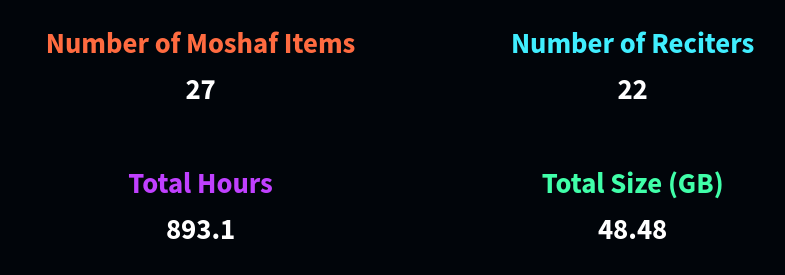
\includegraphics[width=0.8\textwidth]{../figures/stats.png}
\caption{Overview statistics of the collected audio database.}
\label{fig:stats}
\end{figure}

\begin{figure}[H]
\centering
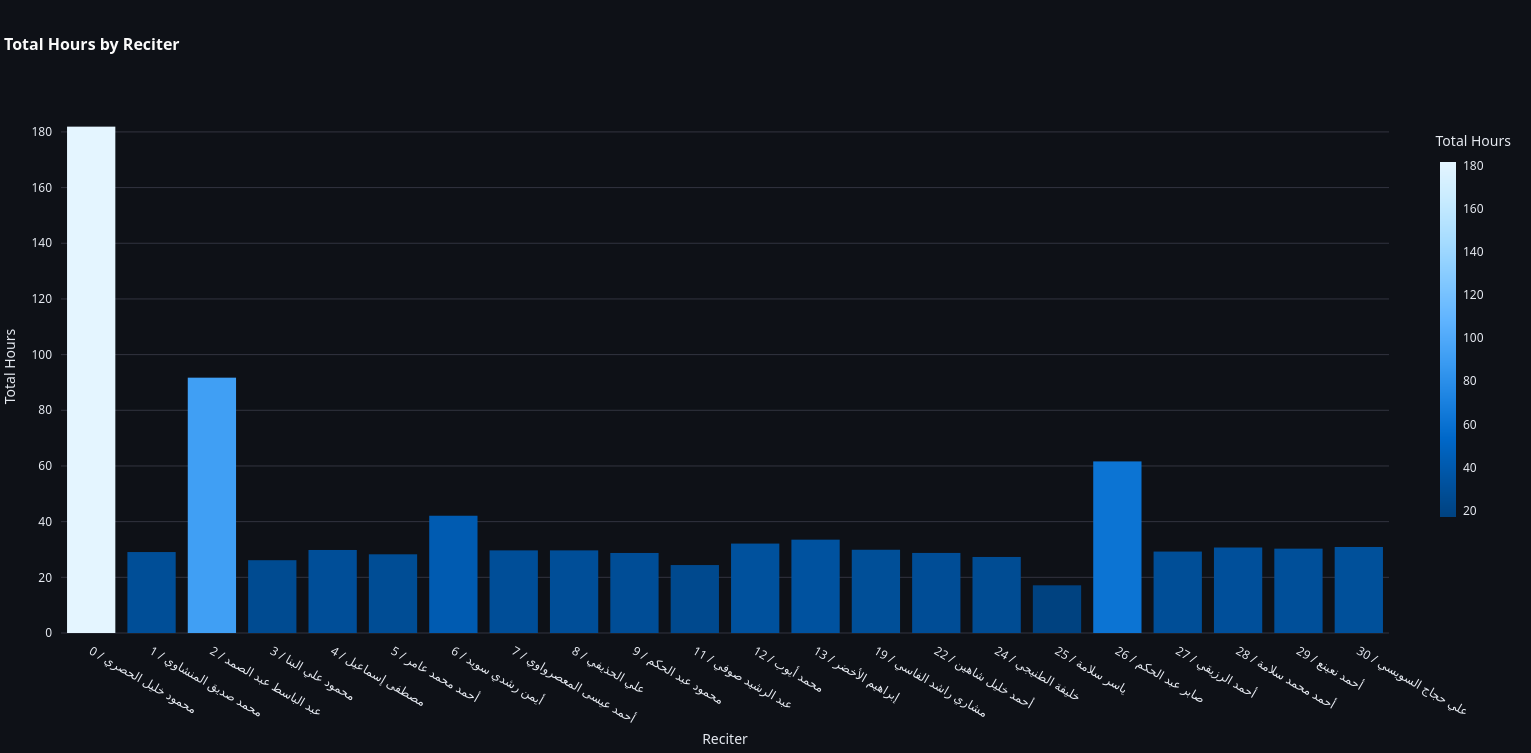
\includegraphics[width=0.8\textwidth]{./figures/reciter.png}
\caption{Total duration of collected recitations, broken down by individual reciter.}
\label{fig:reciter}
\end{figure}

To facilitate this collection, a web GUI was developed using Streamlit\footnote{https://streamlit.io/}. This application performs the following tasks:
\begin{itemize}
\item Downloads audio tracks and extracts their metadata.
\item Organizes the data by Moshaf, with each chapter saved as a separate file (e.g., `001.mp3`).
\item Provides an interface for annotating Moshaf attribute cards.
\end{itemize}

\subsection{Running the Collection Application}

\subsubsection{Cloning the Repository}
The application source code can be obtained by cloning the Git repository:
\begin{lstlisting}[language=bash]
git clone https://github.com/obadx/prepare-quran-dataset
\end{lstlisting}

\subsubsection{Installing `uv`}
The project uses `uv` for dependency management. It can be installed via `pip`:
\begin{lstlisting}[language=bash]
pip install uv
\end{lstlisting}
Alternatively, it can be installed directly from the official installer:
\begin{lstlisting}[language=bash]
curl -LsSf https://astral.sh/uv/install.sh | sh
\end{lstlisting}

\subsubsection{Installing Project Dependencies}
Navigate to the project directory and sync the dependencies, including those for annotation:
\begin{lstlisting}[language=bash]
cd prepare-quran-dataset
uv sync --extra annotate
\end{lstlisting}

\subsubsection{Installing Frontend Dependencies}
The frontend has additional requirements. Navigate to its directory and install them:
\begin{lstlisting}[language=bash]
cd frontend
uv pip install -r requirements.txt
\end{lstlisting}

\subsubsection{Launching the Frontend Application}
With dependencies installed, the Streamlit application can be launched from the `frontend` directory:
\begin{lstlisting}[language=bash]
streamlit run streamlit_app.py
\end{lstlisting}

\subsection{UI Snapshots}

\begin{figure}[H]
\centering
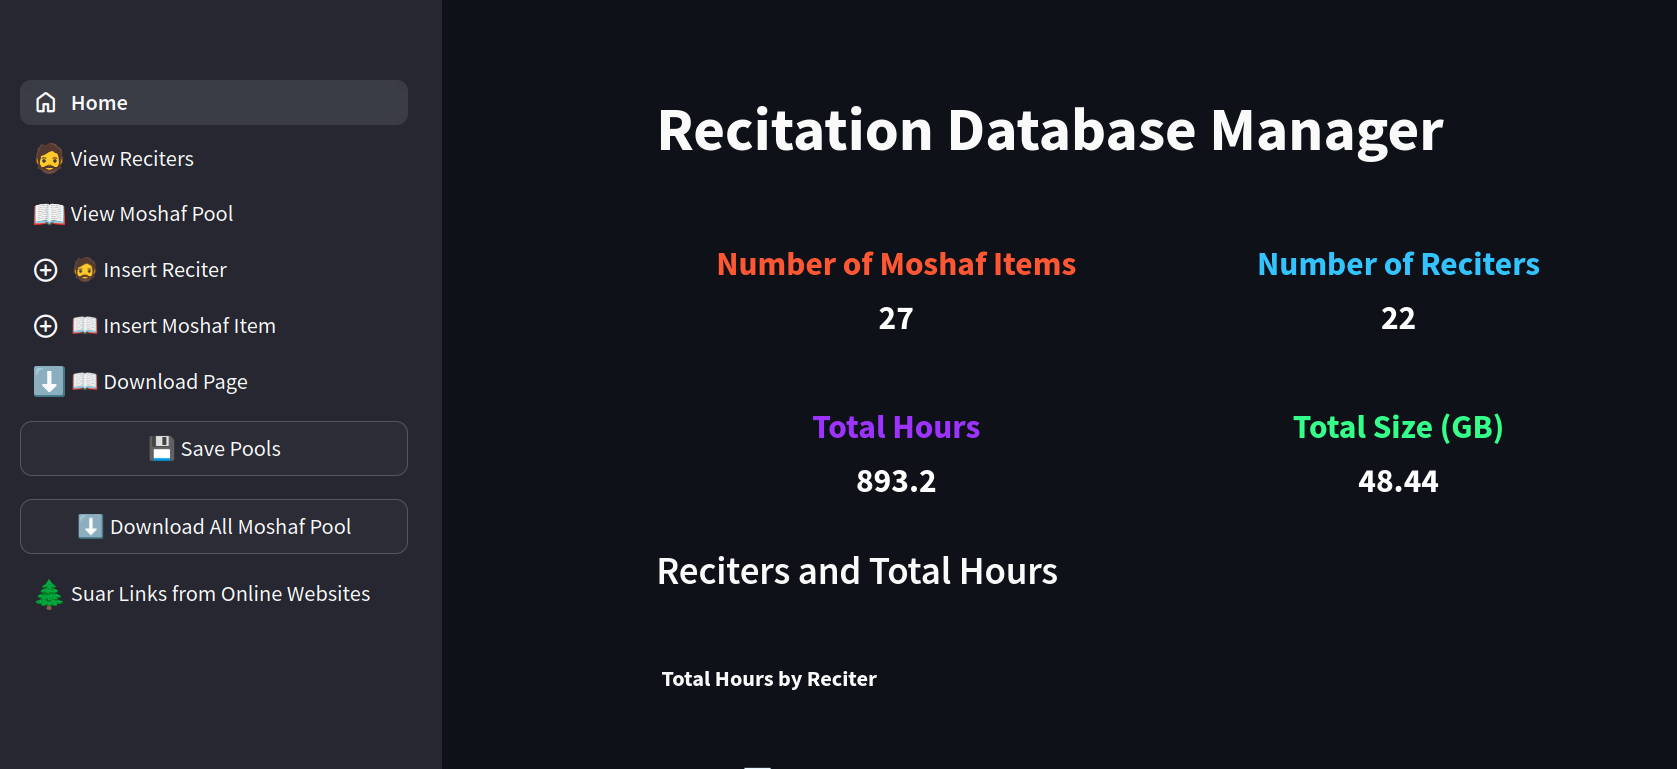
\includegraphics[width=0.8\textwidth]{../figures/ui_main_page.png}
\caption{The main page of the custom annotation platform.}
\label{fig:ui_main}
\end{figure}

\begin{figure}[H]
\centering
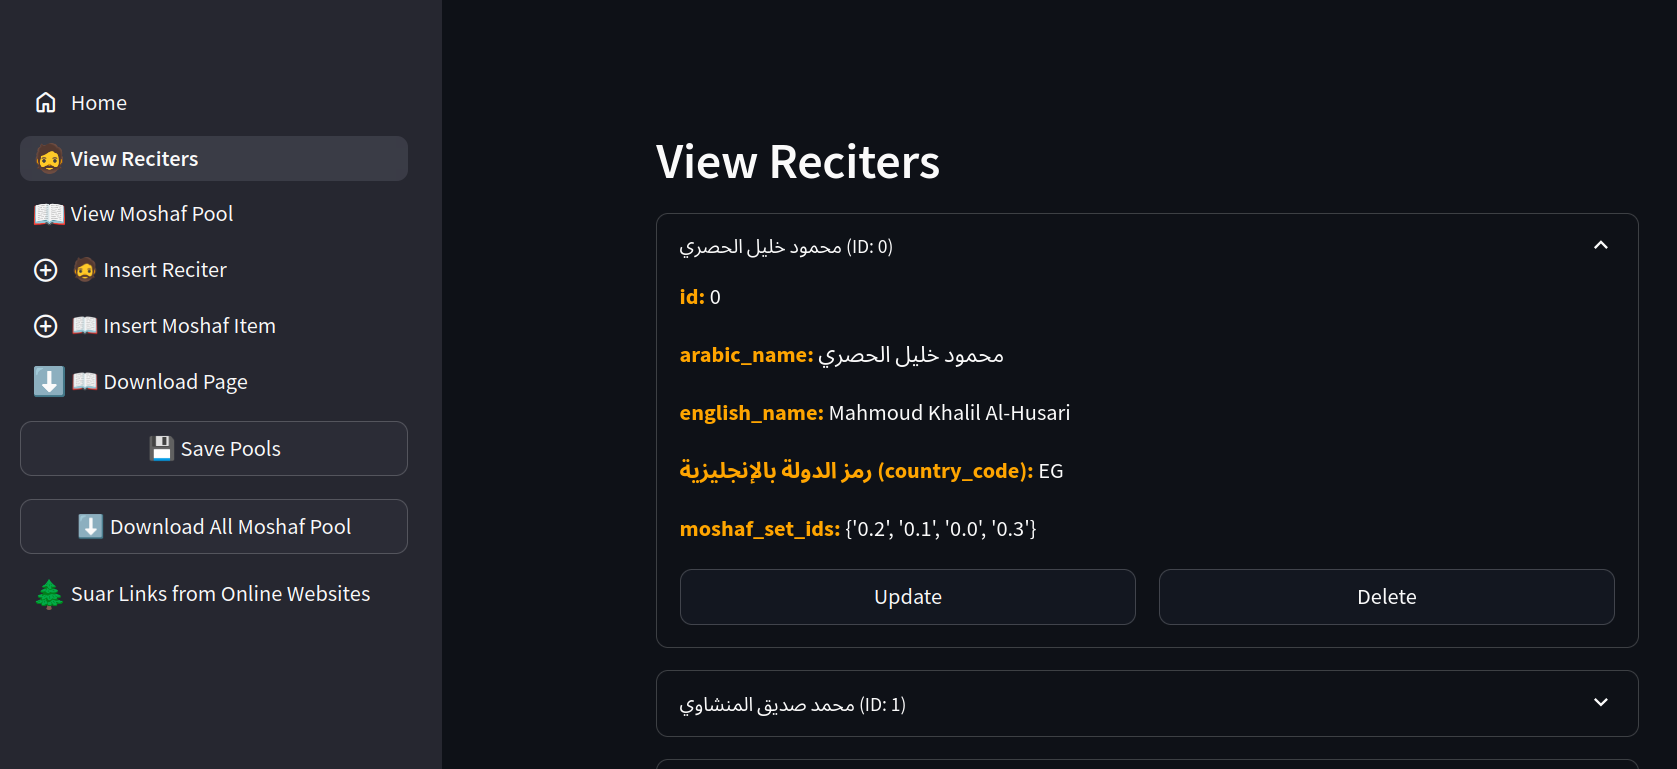
\includegraphics[width=0.8\textwidth]{../figures/ui_veiw_reciters.png}
\caption{The reciter management view within the application.}
\label{fig:ui_reciters}
\end{figure}

\begin{figure}[H]
\centering
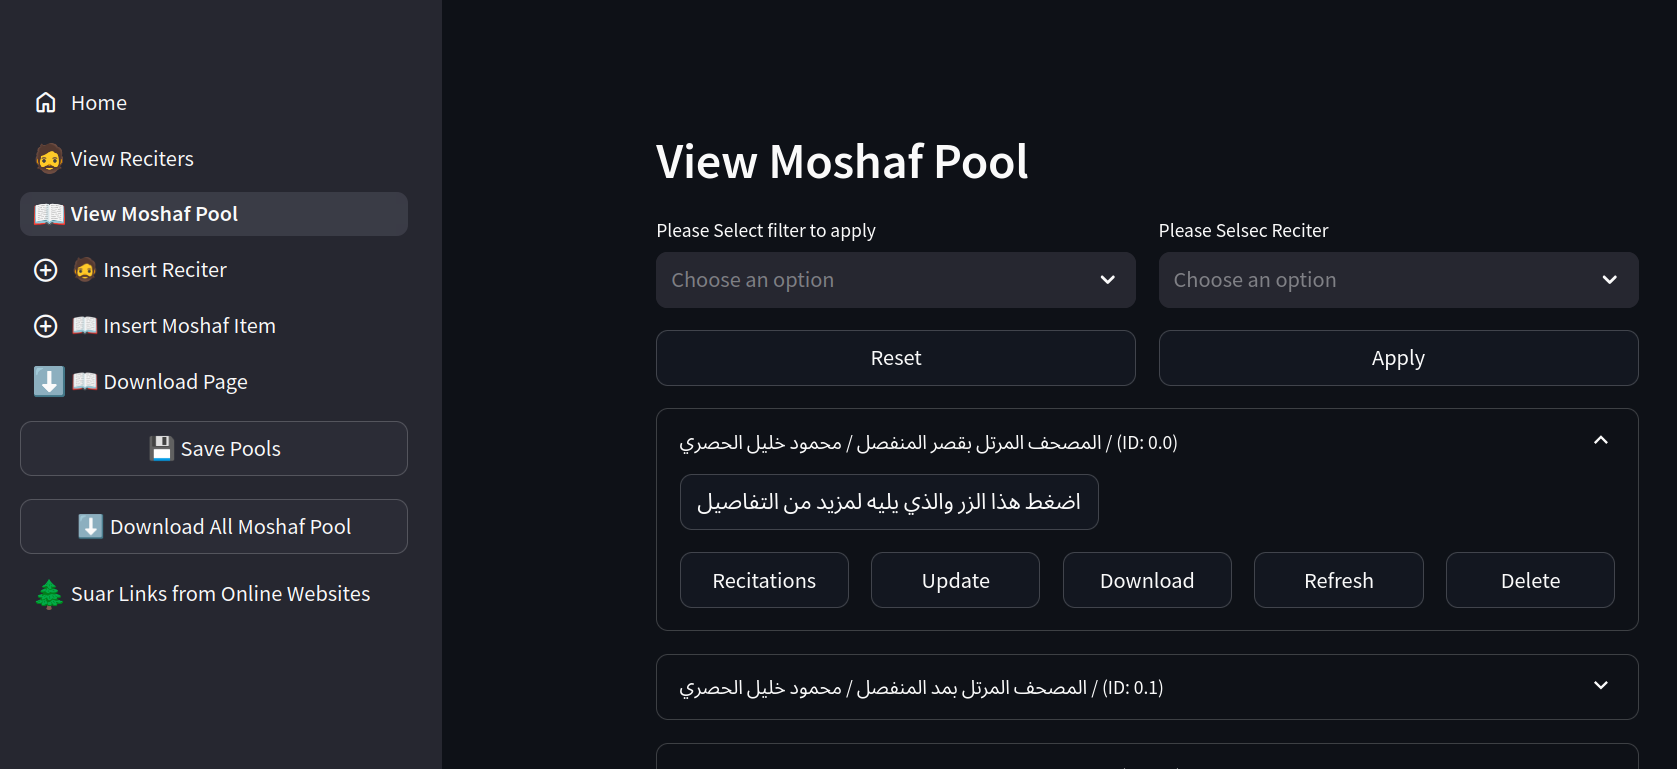
\includegraphics[width=0.8\textwidth]{../figures/ui_veiw_all_moshaf.png}
\caption{View displaying all available Masahif in the database.}
\label{fig:ui_masahif}
\end{figure}

\begin{figure}[H]
\centering
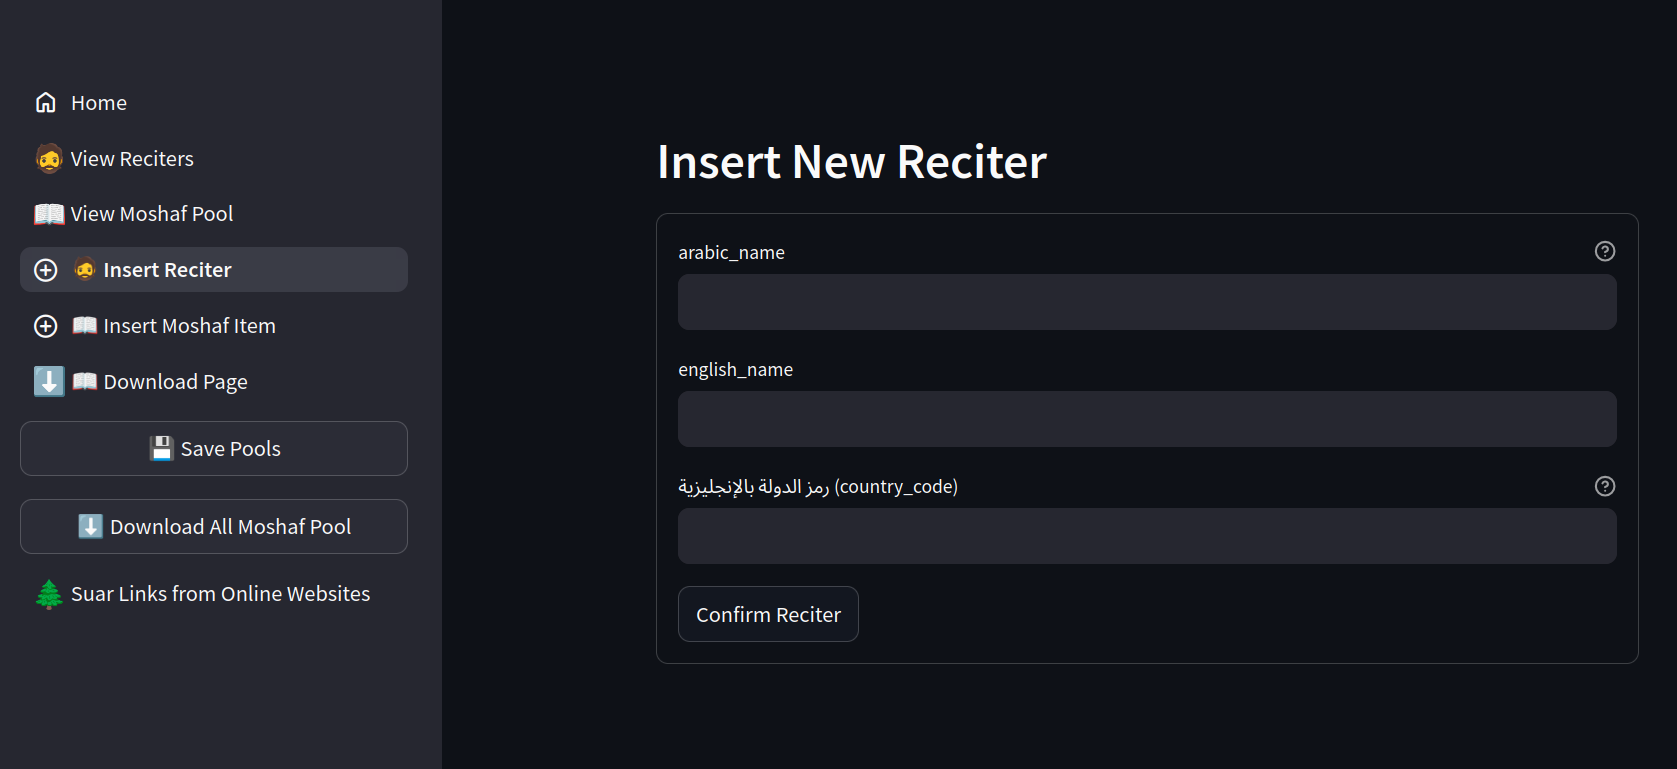
\includegraphics[width=0.8\textwidth]{../figures/ui_insert_new_reciter.png}
\caption{Dialog for inserting a new reciter's details.}
\label{fig:ui_new_reciter}
\end{figure}

\begin{figure}[H]
\centering
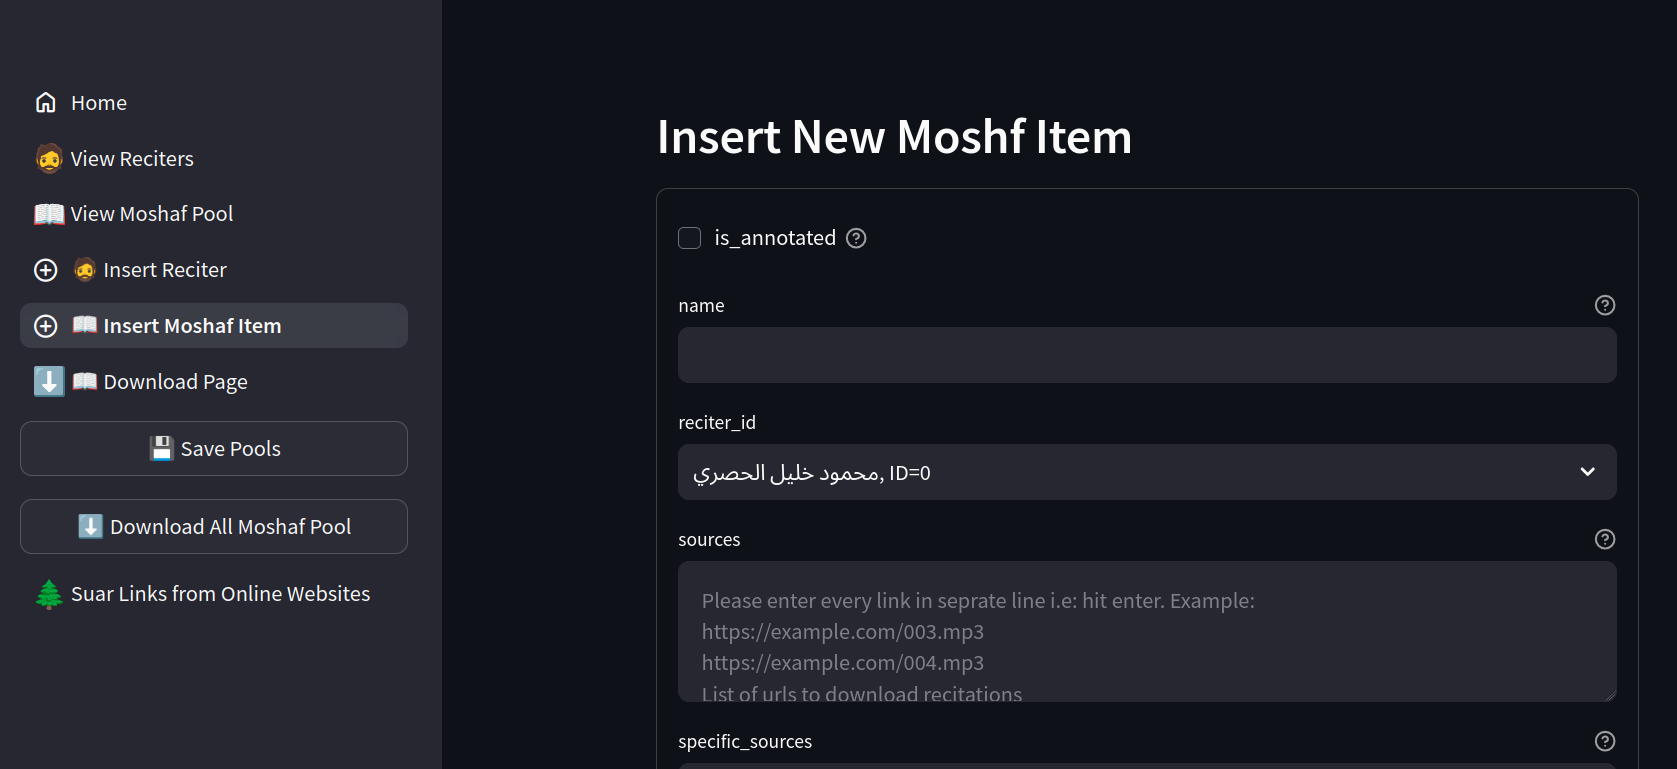
\includegraphics[width=0.8\textwidth]{../figures/ui_inset_new_mohaf.png}
\caption{Dialog for creating and annotating a new Moshaf attribute card.}
\label{fig:ui_new_moshaf}
\end{figure}

\begin{figure}[H]
\centering
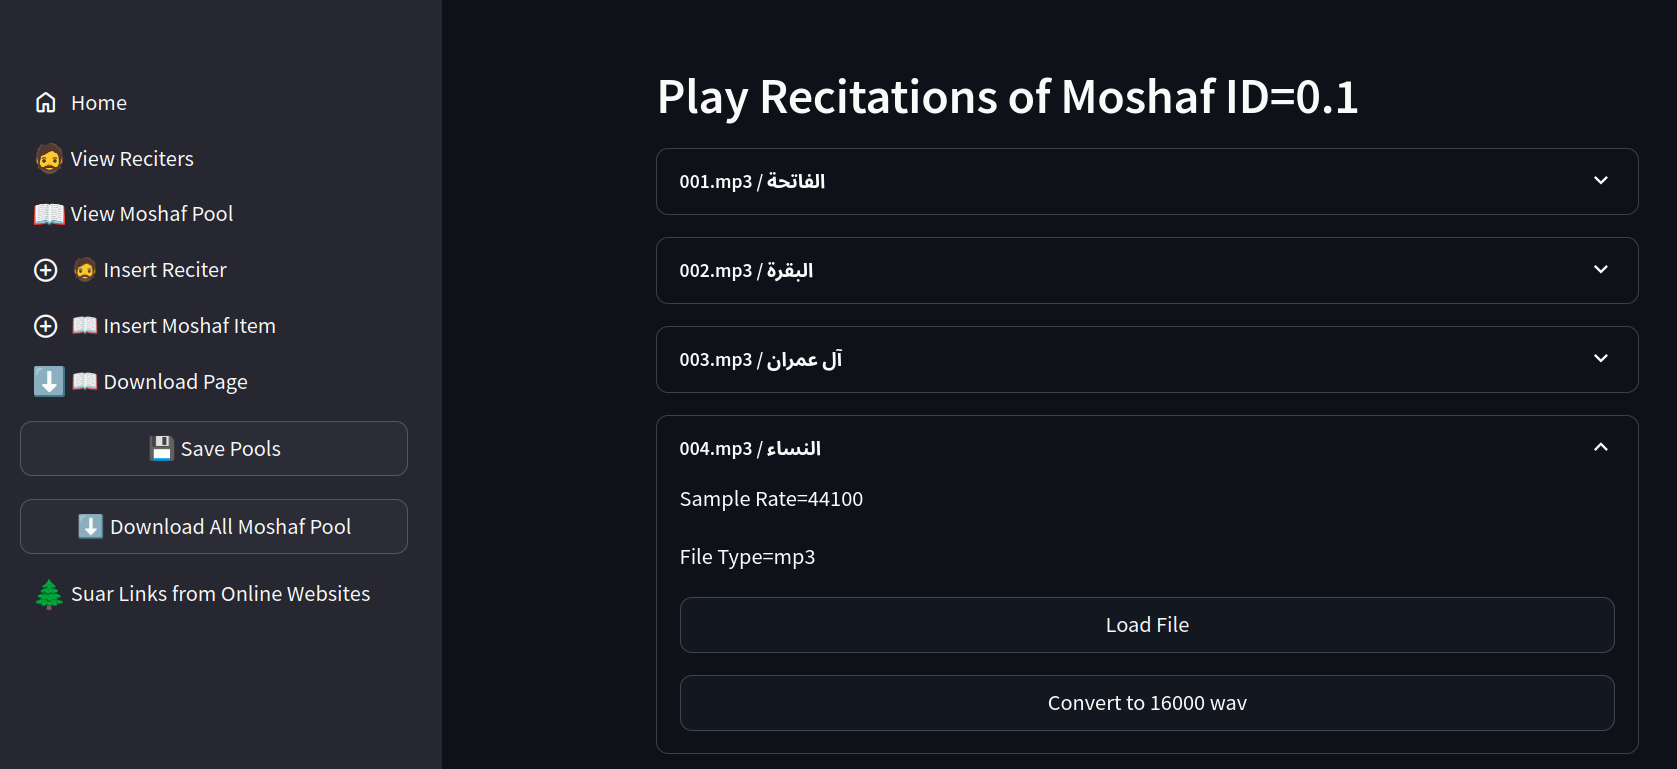
\includegraphics[width=0.8\textwidth]{../figures/ui_play_recitatins.png}
\caption{Interface for viewing a Moshaf's tracks and playing individual recitations.}
\label{fig:ui_play}
\end{figure}






% --------------------------------------------------------



\section{Segmentation of Recitations}

Accurate segmentation is a critical preprocessing step, as Tajweed rules are directly influenced by pause points (\arb{وقف}). To address this, we initially evaluated open-source Voice Activity Detection (VAD) models, including SileroVAD \cite{SileroVAD} and PyAnnotate \cite{Plaquet23}. However, their performance on Quranic recitations was unsatisfactory due to the unique acoustic and prosodic characteristics of Tilawah.

Consequently, we developed a custom segmentation model by fine-tuning the Wav2Vec2-BERT architecture \cite{barrault2023seamless} for frame-level classification, specifically optimized for Quranic audio.

\subsection{Preparation of Segmenter Training Data}

To create a training dataset, we selected \arb{مصاحف} from the EveryAyah\footnote{https://everyayah.com} database that were compatible with SileroVAD v4. This source provided pre-segmented recitations at the verse (ayah) level, which served as our ground truth.

For each Moshaf, we tuned the following segmentation parameters to optimize alignment with the ground truth:
\begin{itemize}
\item \textbf{Threshold:} Detection confidence level.
\item \textbf{Minimum Silence Duration:} Durations below this value trigger segment merging.
\item \textbf{Minimum Speech Duration:} Segments shorter than this value are discarded.
\item \textbf{Padding:} Duration added to the beginning and end of each detected segment.
\end{itemize}

The resulting dataset, comprising eight complete \arb{مصاحف}, is summarized in Table \ref{tab:segmenter_data}.

% \begin{longtable}{|p{4cm}|c|c|c|c|c|c|}
% \caption{Dataset used for training the custom segmenter, consisting of eight complete Masahif with tuned parameters.}
% \label{tab:segmenter_data}\\
% \hline
% \textbf{Reciter Name} & \textbf{ID} & \textbf{Window Size (Samples)} & \textbf{Threshold} & \textbf{Min Silence (ms)} & \textbf{Min Speech (ms)} & \textbf{Pad (ms)} \\ 
% \hline
% \endfirsthead
% \hline
% \arb{محمود خليل الحصري} & 0 & 1536 & 0.3 & 500 & 1000 & 40 \\
% \hline
% \arb{محمد صديق المنشاوي} & 1 & 1536 & 0.3 & 400 & 1000 & 20 \\
% \hline
% \arb{عبد الباسط عبد الصمد} & 2 & 1536 & 0.3 & 400 & 700 & 20 \\
% \hline
% \arb{محمود علي البنا} & 3 & 1536 & 0.3 & 400 & 700 & 20 \\
% \hline
% \arb{على الحذيفي} & 5 & 1536 & 0.3 & 350 & 700 & 5 \\
% \hline
% \arb{أيمن رشدي سويد} & 6 & 1536 & 0.3 & 500 & 1000 & 10 \\
% \hline
% \arb{محمد أيوب} & 7 & 1536 & 0.3 & 400 & 1000 & 10 \\
% \hline
% \arb{إبراهيم الأخضر} & 8 & 1536 & 0.3 & 390 & 700 & 30 \\
% \hline
% \end{longtable}

{\small
\begin{longtable}{|p{2.8cm}|c|c|c|c|c|c|}
\caption{Dataset used for training the custom segmenter, consisting of eight complete Masahif with tuned parameters.}
\label{tab:segmenter_data}\\
\hline
\textbf{Reciter Name} & \textbf{ID} & \textbf{Window Size} & \textbf{Threshold} & \textbf{Min Silence} & \textbf{Min Speech} & \textbf{Pad} \\ 
& & \textbf{(Samples)} & & \textbf{(ms)} & \textbf{(ms)} & \textbf{(ms)} \\ 
\hline
\endfirsthead
\hline
\arb{محمود خليل الحصري} & 0 & 1536 & 0.3 & 500 & 1000 & 40 \\
\hline
\arb{محمد صديق المنشاوي} & 1 & 1536 & 0.3 & 400 & 1000 & 20 \\
\hline
\arb{عبد الباسط عبد الصمد} & 2 & 1536 & 0.3 & 400 & 700 & 20 \\
\hline
\arb{محمود علي البنا} & 3 & 1536 & 0.3 & 400 & 700 & 20 \\
\hline
\arb{على الحذيفي} & 5 & 1536 & 0.3 & 350 & 700 & 5 \\
\hline
\arb{أيمن رشدي سويد} & 6 & 1536 & 0.3 & 500 & 1000 & 10 \\
\hline
\arb{محمد أيوب} & 7 & 1536 & 0.3 & 400 & 1000 & 10 \\
\hline
\arb{إبراهيم الأخضر} & 8 & 1536 & 0.3 & 390 & 700 & 30 \\
\hline
\end{longtable}
}

\subsubsection{Data Augmentation}

To improve model robustness and generalize across various recording conditions, we employed data augmentation using the Audiomentations library. The augmentation strategy replicated SileroVAD's noise profile and was applied to 40\% of the samples. With additional:
\begin{itemize}
\item \texttt{TimeStretch} (0.8x-1.5x) to simulate recitation speeds
\item Sliding window truncation (1-second windows) for long samples instead of exclusion
\end{itemize}

\subsection{Segmenter Training}

The Wav2Vec2BERT model was fine-tuned for frame-level classification over a single epoch. The architecture of our VAD model compared to standard streaming models is illustrated in the figure below.

\begin{figure}[H]
\centering
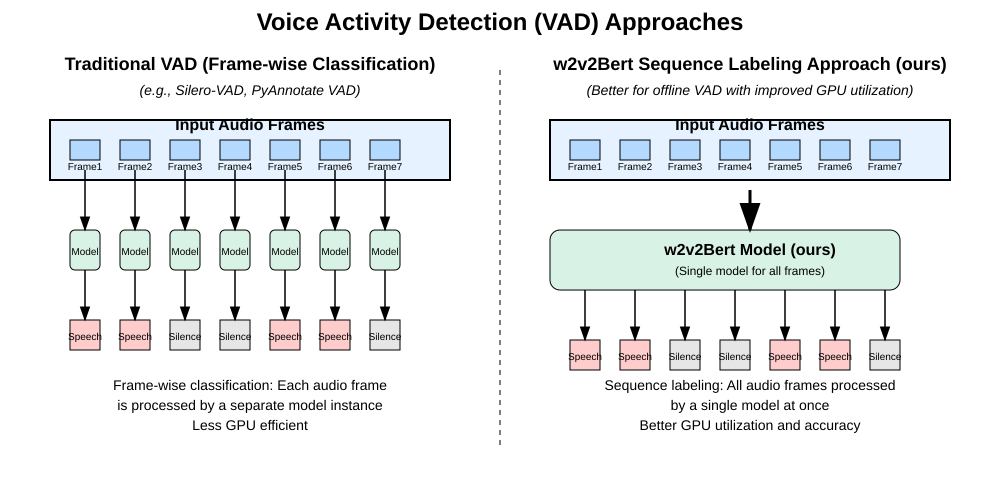
\includegraphics[width=0.8\textwidth]{../figures/vad-arch.png}
\caption{Architecture of the fine-tuned Wav2Vec2-BERT model for frame classification, compared to a standard streaming model.}
\label{fig:vad_arch}
\end{figure}

The model's performance on unseen \arb{مصاحف} demonstrated high accuracy, as shown in Table \ref{tab:vad_results}.

\begin{longtable}{|l|c|}
\caption{Evaluation results of the segmentation model on a held-out test set of Masahif, showing superior performance. The quality of the segmenter was validated by processing our entire dataset, where it maintained this high level of performance. The only exceptions were edge cases involving extremely fast recitation (\arb{حدر}), which is an expected limitation.}
\label{tab:vad_results}\\
\hline
\textbf{Metric} & \textbf{Value} \\ 
\hline
\endfirsthead
\hline
Test Loss & 0.0277 \\
\hline
Test Accuracy & 0.9935 \\
\hline
Test F1 Score & 0.99476 \\
\hline
\end{longtable}






% --------------------------------------------------------------------

\section{Transcribe Segmented Parts}

We employed Tarteel ASR \cite{tarteel_whisper_ar_quran} (Whisper fine-tuned on Quranic recitations \cite{radford2023robust}). To handle its 30-second limit, we used sliding window truncation (10-second windows), with verification in the next step. We used vlLM library because it is really fast thanks to Employing Paged Attention \cite{kwon2023efficient}.





% ------------------------------------------------------------------------





\section{Verification of Segmentation and Transcription}
\section{Data Verification}

To ensure the highest quality of our dataset, we developed a custom verification interface using Streamlit\footnote{https://streamlit.io/}. We manually inspect 50-75 randomly selected samples per Moshaf, focusing on the following aspects:

\begin{itemize}
\item \textbf{Segmentation Quality:} Assessing the accuracy of pause detection to determine if adjustments were needed, including:
\begin{itemize}
    \item Increasing or decreasing padding durations
    \item Merging adjacent segments
    \item Splitting undetected segments
\end{itemize}
\item \textbf{Qalqala (\arb{القلقلة}) Duration Inspection:} Verifying that segments containing Qalqala (\arb{قلقة}) are fully captured without being truncated by brief silences, ensuring the acoustic feature remains intact.
\item \textbf{Hams (\arb{همس}) Duration Inspection:} Similarly checking segments for Hams (a whispered or airy phonation) to ensure the subtle release of air was not missed by the segmenter.
\end{itemize}

\begin{figure}[H]
\centering
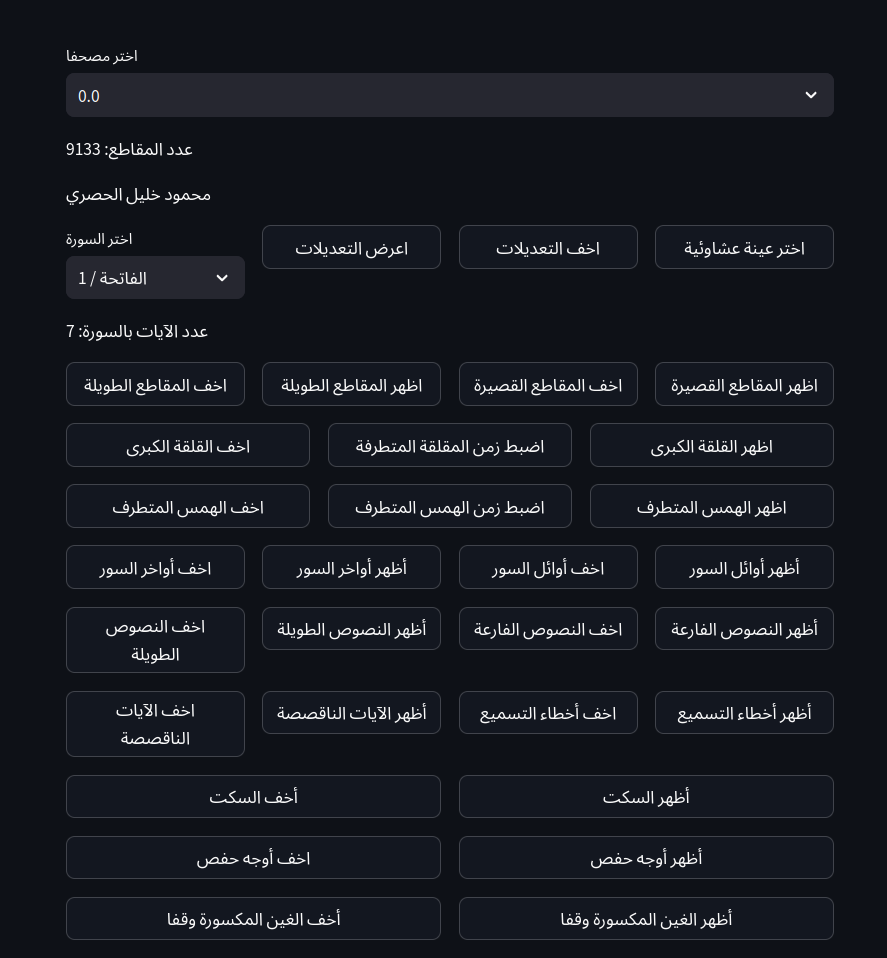
\includegraphics[width=0.8\textwidth]{../figures/data_verfication_ui.png}
\caption{The Streamlit-based UI for manually verifying segmentation quality and phonetic feature integrity.}
\label{fig:verification_ui}
\end{figure}

\begin{figure}[H]
\centering
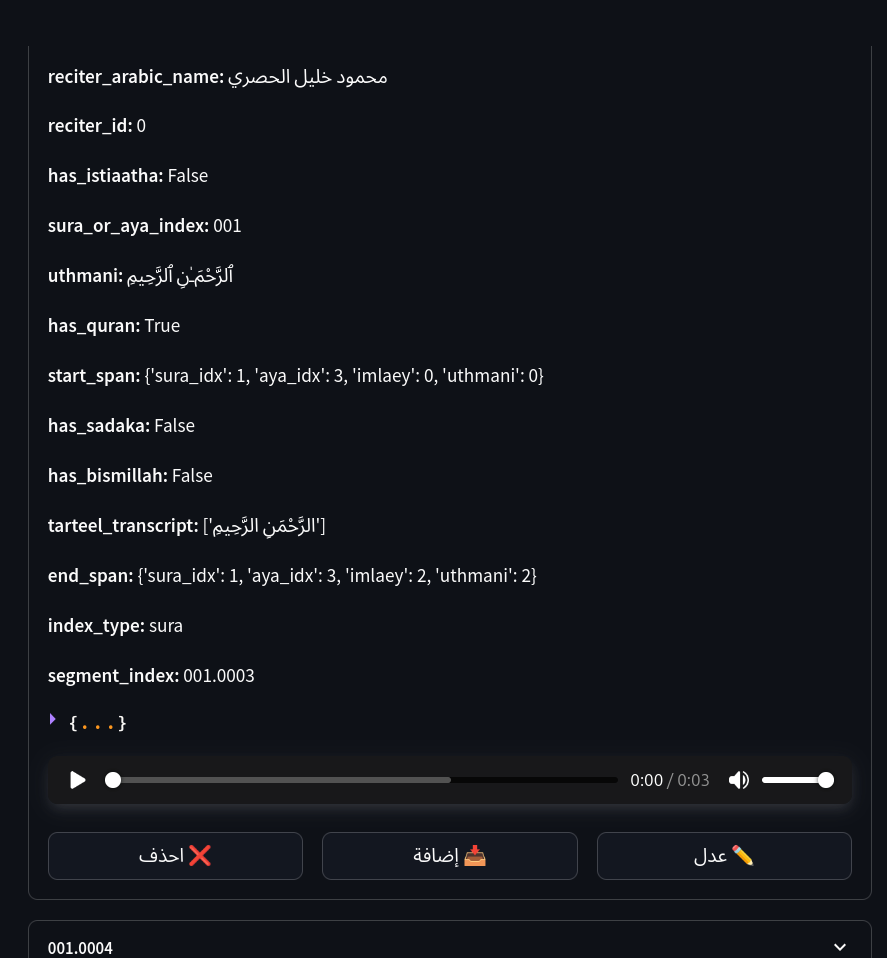
\includegraphics[width=0.8\textwidth]{../figures/data_annotation_ui_editing.png}
\caption{The editing view within the verification UI, allowing for manual correction of segment boundaries.}
\label{fig:annotation_ui}
\end{figure}

After completing the annotation process for a Moshaf, the defined correction operations were programmatically applied to the entire dataset to ensure consistency.

\textbf{Note:} Moshaf 25.0 was excluded from the final dataset due to irreconcilably poor segmentation quality.

\subsection{Transcription Verification: A \arb{تسميع}-Inspired Algorithm}

To validate the accuracy of the automated speech recognition (ASR) output, we developed a verification algorithm inspired by Tasmeea (\arb{تسميع})—the traditional practice where a student recites for a teacher to correct mistakes. This statistical algorithm operates under the core assumption that the input recitations are 100\% correct, and any errors originate from the ASR model (Tarteel model).

The algorithm proceeds through the following steps:
\begin{enumerate}
\item \textbf{Automatic Matching:} Segments are automatically matched to the canonical Quranic text.
\item \textbf{Discrepancy Identification:} The system identifies missing verses, words, or unexpected additions in the transcription.
\item \textbf{Manual Correction:} flagged discrepancies are presented for manual review and correction within our annotation UI, completing the \arb{تسميع} feedback loop.
\end{enumerate}
















\begin{algorithm}[H]
\caption{Tasmeea Algorithm}
\label{alg:tasmeea}
\begin{algorithmic}[1]
\REQUIRE $text\_segments = [s_1, s_2, \dots, s_n]$, $sura\_idx$, 
          $overlap\_words = 6$, $window\_words = 30$, 
          $acceptance\_ratio = 0.5$, flags for special phrases
\ENSURE List of tuples $(match, ratio)$ per segment

\STATE $aya \leftarrow 1$ \COMMENT{Start at first verse}
\STATE $penalty \leftarrow 0$
\FOR{each segment $s_i$ in $text\_segments$}
    \STATE $norm\_text \leftarrow$ normalize($s_i$) \COMMENT{Remove spaces/diacritics}
    \STATE $min\_win \leftarrow window\_words - 10$, $max\_win \leftarrow window\_words + 10$
    \STATE $start\_range \leftarrow [-(overlap + penalty), (overlap + \max(window\_words, max\_win) + penalty]$
    
    \IF{first segment \AND $include\_istiaatha$}
        \STATE Check istiaatha special case
    \ELSIF{last segment \AND $include\_sadaka$}
        \STATE Check sadaka special case
    \ENDIF
    
    \STATE $best\_ratio \leftarrow 0$, $best\_match \leftarrow \text{null}$
    \FOR{each start position $p$ in $start\_range$}
        \FOR{each window size $w \in [min\_win, max\_win]$}
            \STATE $c \leftarrow$ extract candidate at ($aya$, $p$, $w$)
            \STATE $dist \leftarrow \text{edit\_distance}(norm\_text, c)$
            \STATE $ratio \leftarrow 1 - \min(dist, |norm\_text|) / |norm\_text|$
            \IF{$ratio > best\_ratio$ \OR ($ratio = best\_ratio$ \AND $|p| < |best\_start|$)}
                \STATE update $best\_ratio$, $best\_match$, $best\_start$, $best\_window$
            \ENDIF
        \ENDFOR
    \ENDFOR
    
    \IF{$best\_ratio < acceptance\_ratio$}
        \STATE output (null, $best\_ratio$)
        \STATE $penalty \leftarrow max\_win$
        \STATE $aya \leftarrow aya + 1$ \COMMENT{Default advance}
    \ELSE
        \STATE output ($best\_match$, $best\_ratio$)
        \STATE $aya \leftarrow aya + best\_start + best\_window$
        \STATE $penalty \leftarrow 0$
    \ENDIF
\ENDFOR
\STATE \textbf{Complexity:} $O(N \cdot W \cdot L^2)$ \COMMENT{$N$=segments, $W$=window size, $L$=segment length}
\end{algorithmic}
\end{algorithm}
 
% Chapter Template

\chapter{Modeling Quran Phonetic Script} % Main chapter title

\label{Chapter5} % Change X to a consecutive number; for referencing this chapter elsewhere, use \ref{ChapterX}

\lhead{Chapter 5. \emph{Modeling Quran Phonetic Script}} % Change X to a consecutive number; this is for the header on each page - perhaps a shortened title




\section{Modeling}

Our Quran Phonetic Script produces two types of outputs: `phonemes` and `sifat` (which comprises 10 distinct attributes). We model this task as follows: Imagine processing an input speech utterance and simultaneously generating transcripts in multiple languages, such as Arabic, English, French, and German. Similarly, we implement a speech encoder with a separate linear output layer for each of our 11 levels (one for `phonemes` and 10 for the `sifat` attributes), resulting in 11 parallel transcription heads. We employ the Connectionist Temporal Classification (CTC) loss \cite{graves2006ctc} without a language model, as our objective is to transcribe the actual pronunciation rather than the intended utterance. We refer to this architecture as \textbf{Multi-level CTC}.

The total loss is computed as a weighted average of the CTC losses across all 11 levels. The `phonemes` level is assigned a weight of 0.4 due to its larger vocabulary size (43 symbols), while the remaining levels are weighted proportionally lower:

\begin{equation}
\text{loss} = \sum_{i} \left( \text{level\_weight}_i \cdot \text{CTC\_level}_i \right)
\label{eq:multilevel_ctc}
\end{equation}

We used a weight of 0.4 for the `phonemes` level, 0.0605 for both `shidda_or_rakhawa` and `tafkheem_or_taqeeq`, and 0.059875 for each of the remaining levels.

\begin{figure}[H]
\centering
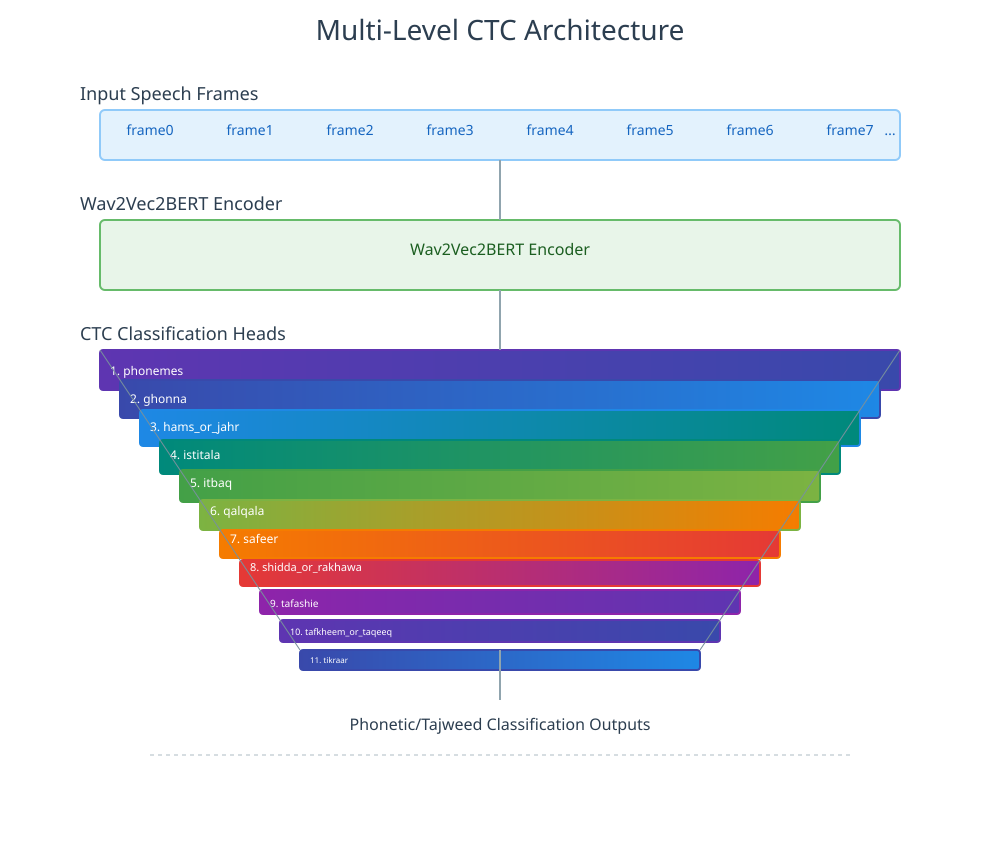
\includegraphics[width=0.8\textwidth]{../figures/multi-level-ctc.png}
\caption{Multi-level CTC architecture with 11 output heads, each computing a CTC loss, combined via weighted average.}
\label{fig:multi_level_ctc}
\end{figure}

We fine-tuned Facebook's Wav2Vec2-Bert model \cite{barrault2023seamless} for a single epoch using a constant learning rate of \texttt{5e-5}. Data augmentations were applied using the \texttt{audiomentations} library \cite{Audiomentations}, mirroring the augmentations used in Silero VAD \cite{SileroVAD}, with additional augmentations including \texttt{TimeStretch} and \texttt{GainTransition}. Samples longer than 30 seconds were filtered out to optimize GPU memory utilization—this resulted in the exclusion of only 3k samples from the 250k training set.

\begin{figure}[H]
\centering
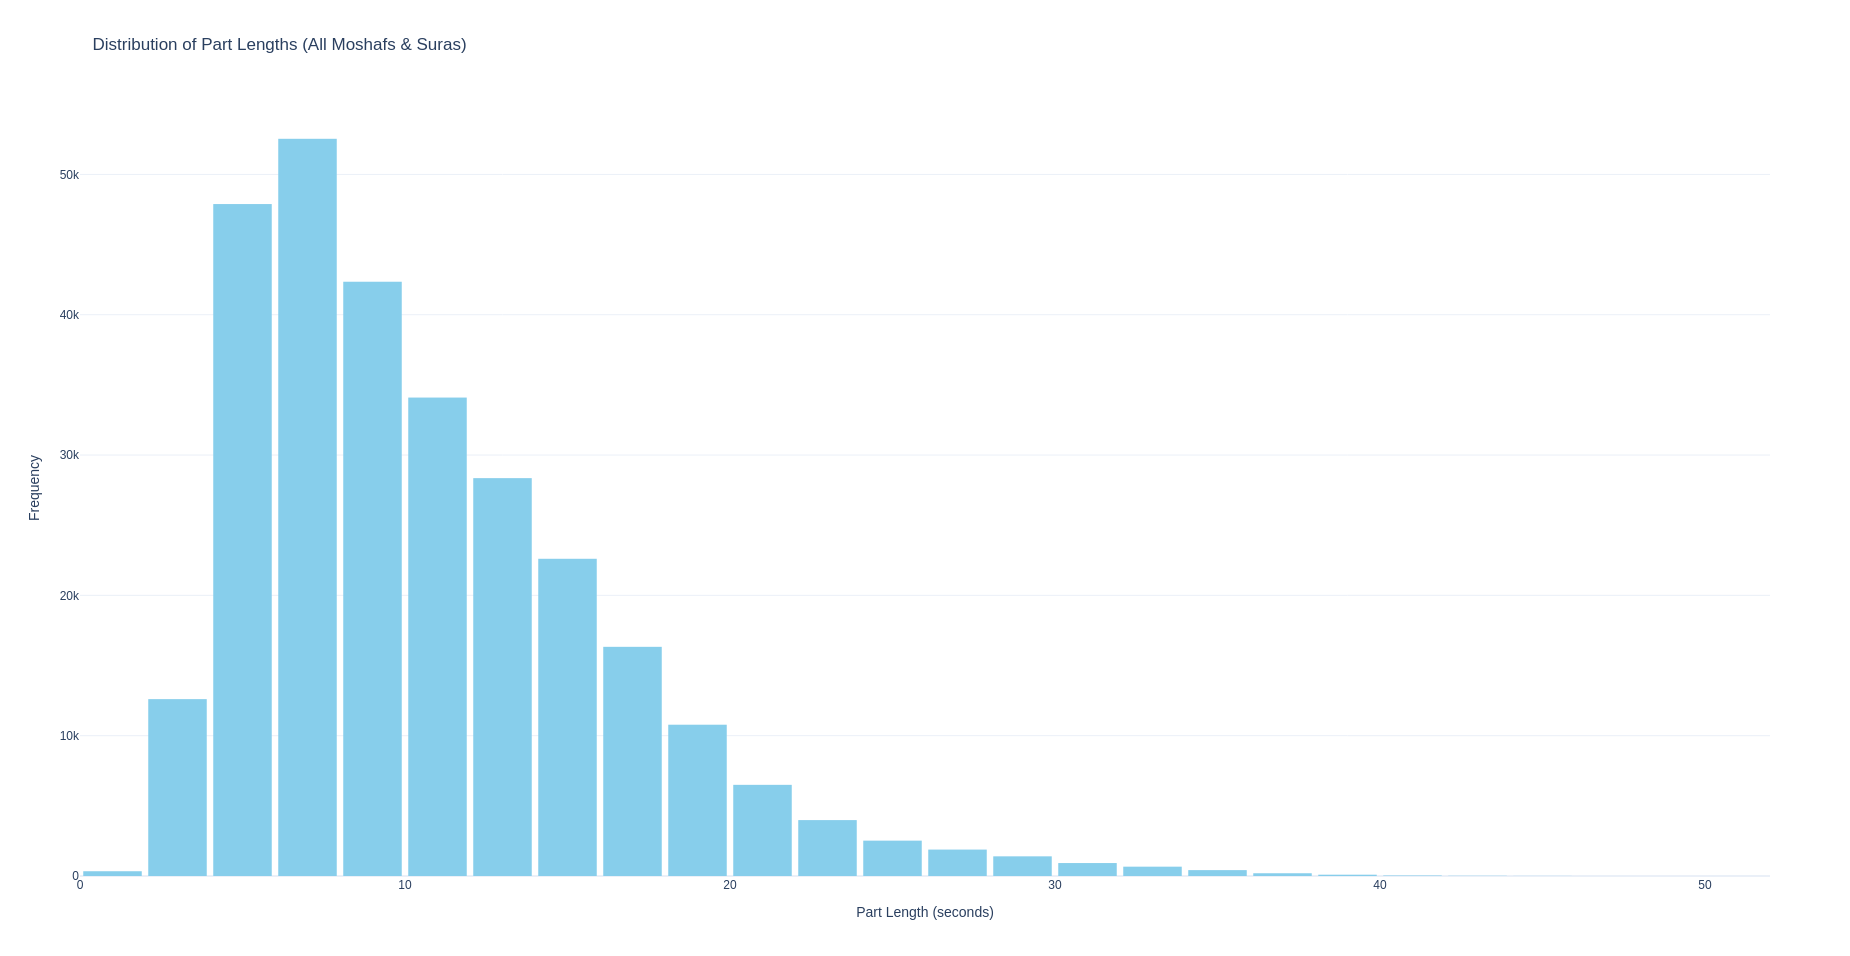
\includegraphics[width=0.8\textwidth]{./figures/audio-lens.png}
\caption{Distribution of recitation lengths (in seconds) across the dataset.}
\label{fig:audio_lens}
\end{figure}

Training was conducted on a single H200 GPU with 141 GB of memory and completed in approximately 7 hours.
 
% Chapter Template

\chapter{Results} % Main chapter title

\label{Chapter6} % Change X to a consecutive number; for referencing this chapter elsewhere, use \ref{ChapterX}

\lhead{Chapter 6. \emph{Results}} % Change X to a consecutive number; this is for the header on each page - perhaps a shortened title




\section{Results}

We trained our model on all available Mushaf recitations, reserving Mushaf 26.1 and 19.0 exclusively for testing. The evaluation results are summarized in Table \ref{tab:results}. The achieved Average Phoneme Error Rate (PER) of 0.16\% strongly supports our hypothesis that the Quran Phonetic Script is learnable using modern speech processing techniques.

We further tested the model on actual samples containing errors in \arb{مد}, \arb{غنة}, \arb{قلقلة}, and \arb{تفخيم}. Despite being trained only on error-free expert recitations, the model successfully detected these common pronunciation mistakes. While these preliminary results are promising, a more comprehensive evaluation on dedicated error-annotated datasets—such as \cite{khan2021tarteel}—is planned for future work.

We observe that the PER is well-balanced across nearly all phonetic and attribute levels, with the exception of the phoneme level itself. This is expected, as the phoneme level has a significantly larger vocabulary (44 symbols, including padding), increasing its complexity relative to the attribute levels.


\begin{table}[htbp]
\centering
\caption{Test results on Mushaf 26.1 and 19.0. The Average Phoneme Error Rate (PER) is \textbf{0.16\%}, confirming the learnability of the Quran Phonetic Script. The phoneme-level PER is higher (0.54\%) due to its larger vocabulary.}
\label{tab:results}\\
\vspace{3pt}
\label{tab:results}
\begin{tabular}{lc}
\hline
\textbf{Metric} & \textbf{Value} \\
\hline
loss & 0.01162 \\
per\_phonemes & 0.00543 \\
per\_hams\_or\_jahr & 0.00117 \\
per\_shidda\_or\_rakhawa & 0.00172 \\
per\_tafkheem\_or\_taqeeq & 0.00167 \\
per\_itbaq & 0.00092 \\
per\_safeer & 0.00132 \\
per\_qalqla & 0.00085 \\
per\_tikraar & 0.0009 \\
per\_tafashie & 0.0016 \\
per\_istitala & 0.0008 \\
per\_ghonna & 0.0013 \\
average\_per & \textbf{0.0016} \\
\hline
\end{tabular}
\end{table}


To evaluate real-world performance, we developed a demonstration application using Gradio\footnote{https://www.gradio.app/}. The interface allows users to record or upload their recitations and receive immediate phonetic and attribute-level feedback.

\begin{figure}[H]
\centering
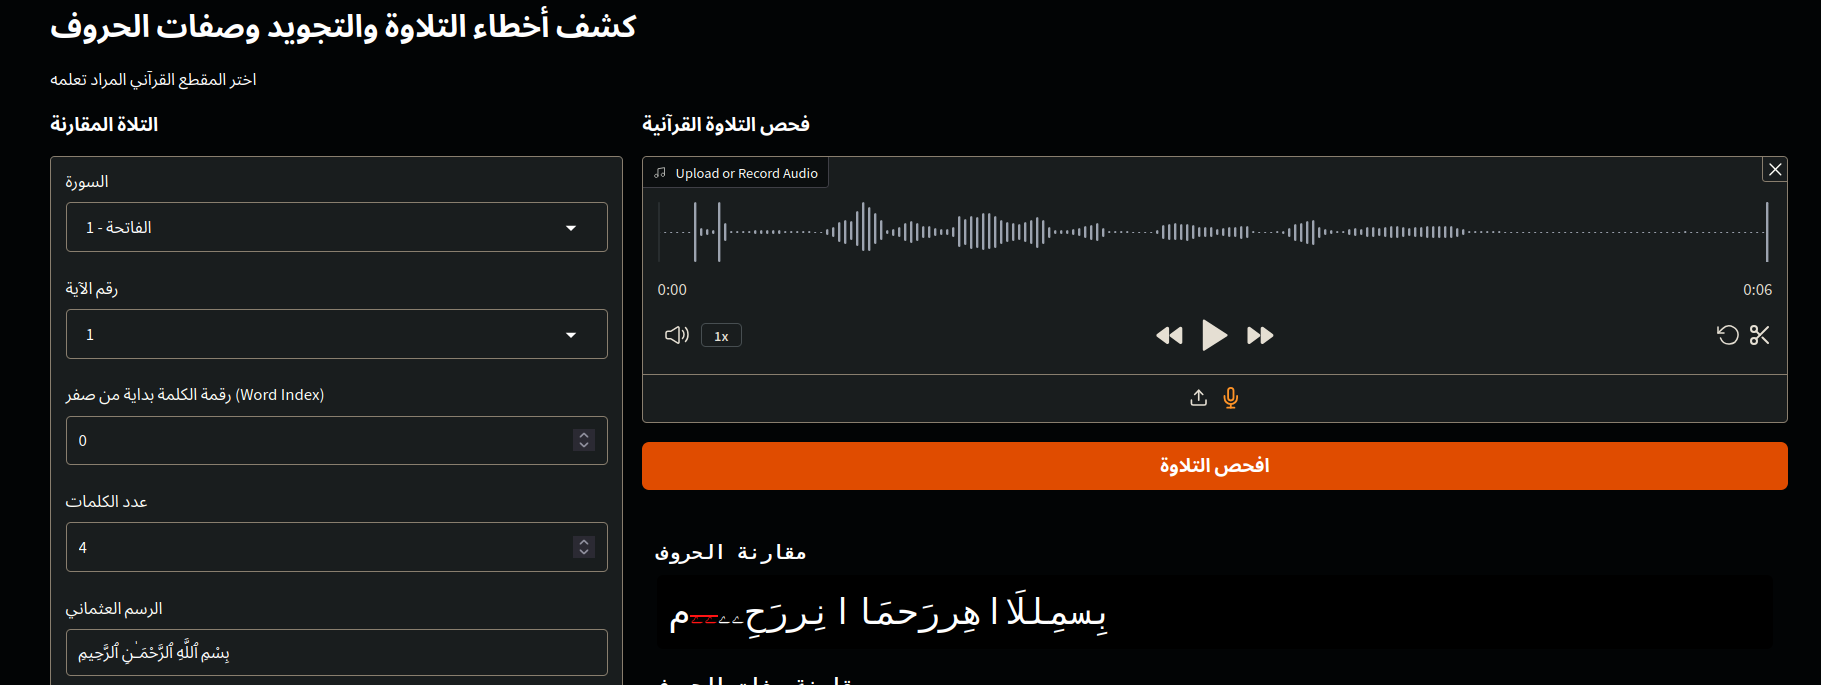
\includegraphics[width=0.8\textwidth]{../figures/gradio_ui_main.png}
\caption{Gradio Web App interface allowing users to test our model.}
\label{fig:gradio_main}
\end{figure}

\begin{figure}[H]
\centering
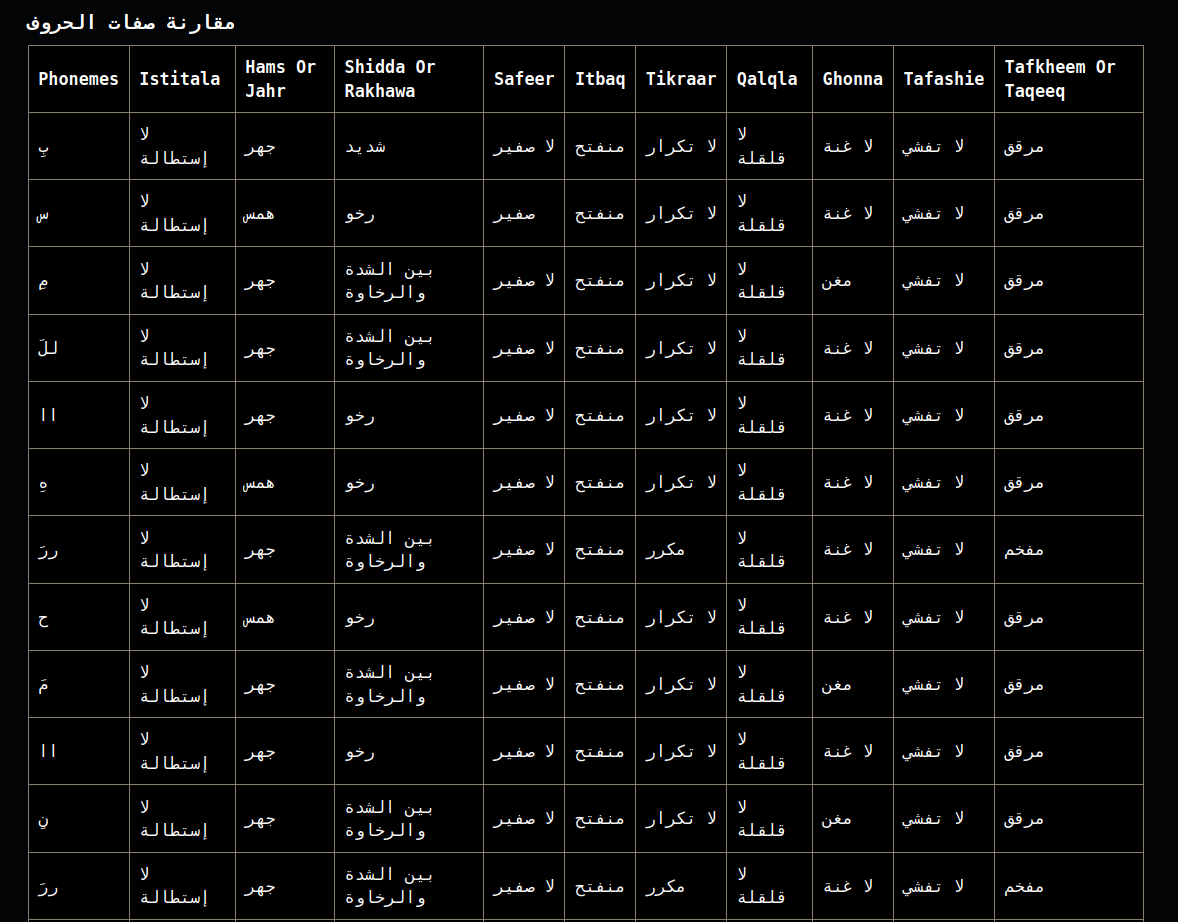
\includegraphics[width=0.8\textwidth]{../figures/gradio_ui_sifa.png}
\caption{Gradio Web App interface showing detailed Sifat (attribute) level feedback.}
\label{fig:gradio_sifa}
\end{figure}

User feedback has been extremely positive. Notably, the model generalized well to female voices despite being trained exclusively on male recitations, successfully detecting common errors such as incorrect \arb{مد} elongation or weak \arb{قلقلة} pronunciation. This demonstrates the robustness and practical applicability of our approach.
 
% Chapter Template

\chapter{Conclusion} % Main chapter title

\label{Chapter7} % Change X to a consecutive number; for referencing this chapter elsewhere, use \ref{ChapterX}

\lhead{Chapter 7. \emph{Conclusion}} % Change X to a consecutive number; this is for the header on each page - perhaps a shortened title

\section*{Conclusion}

We present a new way of assessing pronunciation errors of Holy Quran learners by developing multi-level Quran Phonetic Script capable of capturing all pronunciation errors for \arb{حفص} except for \arb{إشمام} (as it is a sign not pronounced by mouth), along with 890 hours and 300K of annotated data, a 98\% pipeline to create similar data, plus modeling and validation \cite{citation}.


\section{Limitations}

Our primary limitation is that our dataset consists of golden recitations with no errors, limiting our ability to evaluate performance on real-world data. Although we tested on a few actual samples and successfully detected \arb{مد}, \arb{غنة}, and \arb{قلقة} errors, we need to develop a comprehensive dataset containing error-containing recitations transcribed with our Quran Phonetic Script.

A secondary limitation arises from attribute-specific articulation patterns: Certain attributes apply exclusively to individual letters, such as `Istitala` for (\arb{ض}) and `Tikrar` for (\arb{ر}). Consequently, we expect our model will be unable to capture instances of (\arb{ض}) without `Istitala` or (\arb{ر}) without `Tikrar`. This limitation similarly applies to Tajweed rules that occur less frequently in the Holy Quran, such as \arb{إمالة}, \arb{روم}, and \arb{تسهيل}.

\section{Future Work}

To address these limitations, we plan to:

\begin{enumerate}
\item \textbf{Develop an Error-Included Dataset:}
Collect and annotate a large-scale dataset of learner recitations containing common Tajweed errors, transcribed using our phonetic script. This will enable more robust model training and evaluation.

\item \textbf{Expand to Other Recitation Styles (\arb{روايات}):}
Extend the phonetic script and modeling framework to support additional recitation styles (e.g., \arb{ورش} or \arb{قالون}), facilitating broader applicability across the Muslim world.

\item \textbf{Deploy and Evaluate in Real-World Settings:}
Integrate the model into user-friendly applications and evaluate its effectiveness in real-world learning environments, incorporating feedback from Quran teachers and students to iteratively improve the system.
\end{enumerate}

By addressing these challenges, we aim to advance the state of Quranic pronunciation assessment and make automated, accurate feedback accessible to learners worldwide.

 


\addtocontents{toc}{\vspace{2em}} % Add a gap in the Contents, for aesthetics

%\backmatter

%----------------------------------------------------------------------------------------
%	BIBLIOGRAPHY
%----------------------------------------------------------------------------------------
\cleardoublepage
\label{Bibliography}
\renewcommand{\bibname}{References}
\phantomsection
\addtotoc{References}
\lhead{\emph{References}} % Change the page header to say "References"

\bibliographystyle{unsrtnat} % Use the "unsrtnat" BibTeX style for formatting the Bibliography

\bibliography{Bibliography} % The references (bibliography) information are stored in the file named "Bibliography.bib"

%----------------------------------------------------------------------------------------
%	THESIS CONTENT - APPENDICES
%----------------------------------------------------------------------------------------

% \addtocontents{toc}{\vspace{2em}} % Add a gap in the Contents, for aesthetics

% \appendix % Cue to tell LaTeX that the following 'chapters' are Appendices

% Include the appendices of the thesis as separate files from the Appendices folder
% Uncomment the lines as you write the Appendices

% % Appendix A

\chapter{Appendix Title Here} % Main appendix title

\label{AppendixA} % For referencing this appendix elsewhere, use \ref{AppendixA}

\lhead{Appendix A. \emph{Appendix Title Here}} % This is for the header on each page - perhaps a shortened title

Write your Appendix content here.
%\input{Appendices/AppendixB}
%\input{Appendices/AppendixC}



\end{document}  
